\documentclass[british,         % thesis language
% ngerman
BCOR=2mm,                       % binding correction for printing (ca. 1mm per 10 pages for hardcover binding)
11pt,                           % font size
a4paper,						% page layout
oneside,						% oneside/twoside option for printing
cdgeometry=centered,            % setting of page geometry (format, height, page margins; set to 'cdgeometry=false' for individual type area calculation by package 'typearea'
toc=chapterentrydotfill,        % dots in table of contents
toc=indent,                     % indentation of toc items
bibliography=totoc,         	% bibliography to table of contents
listof=totoc,                   % lists to table of contents
numbers=noenddot,				% last number in table of contents without dot
parskip=full,                   % line break with a free line
cdfont=true
%cdmath=false					% regular font in math mode
]{tudscrreprt}                  % document class ('tudscrreprt' in most cases)

\headlogo[]{figures/EE2_logo.png}
\iftutex
\usepackage{fontspec}
\else
\usepackage[T1]{fontenc}
\usepackage[ngerman=ngerman-x-latest]{hyphsubst}
\fi
\usepackage{isodate}

%% ****************************************************************
%% Packages
%% ****************************************************************

% basic packages

%% set language (german or english)
%% Note that the choice of language for babel only determines the language of chapter titles and paper formalia which are defined in the tudscr package.
%\usepackage[ngerman]{babel}
\usepackage[british]{babel}

\usepackage{geometry}                       % definition of individual page style/geometry
\usepackage{setspace}                   	% line spacing 
\usepackage{enumitem}	                    % enumerations
\usepackage[hyphens]{url}                   % line break at a slash in urls
\usepackage[headsepline]{scrlayer-scrpage}  % head and foot notes
\usepackage{mathptmx}                       % sets Times New Roman for math
\usepackage{amsmath}                        % mathematical equations
%\setlength\mathindent{0pt}
\usepackage[gen]{eurosym}                   % for € symbol
\usepackage{microtype}                      % for several typographical details
\usepackage[pdfborder={0 0 0}]{hyperref}    % for links in the document
\usepackage[output-decimal-marker={.}]{siunitx} % definition of units, displayed with decimal point; may change decimal separator to "," for german language
\usepackage[nohyperlinks]{acronym}	        % for abbreviations list and makros
\usepackage{listings}                       % for code listings
\usepackage{xcolor}                         % definition of colors for highlighting, drawings, ...
\definecolor{codegray}{rgb}{0.5,0.5,0.5}    % background color for code listings
\usepackage{scrhack}                        % avoids warnings for deprecated packages

% packages for tables and graphics
\usepackage{circledsteps}
\usepackage{placeins}
\usepackage{graphicx}                       % import of graphical elements (png, pdf, ...)
\usepackage{hvfloat}	                    % rotating tables and pictures
\usepackage[countmax]{subfloat}             % arrangement of two tables/figures in one environment
\usepackage{here}
\usepackage{multirow}                       
\usepackage{multicol}      
\usepackage{tabularx}
\usepackage{diagbox}
\usepackage{makecell}
\usepackage{colortbl}
\usepackage{threeparttable}

%\usepackage{showframe}                     % displays page margins, ...

\newcolumntype{C}[1]{>{\centering\arraybackslash}m{#1}} % new centered column type
\newcolumntype{L}[1]{>{\arraybackslash}m{#1}}

\usepackage[labelfont=bf, singlelinecheck=off]{caption} % global settings for figure and table captions
\captionsetup[figure]{justification=raggedright}
\captionsetup[table]{justification=raggedright}
\DeclareCaptionType{listing}[Listings][List of Listings] % definition of new environment with title for toc




%% ****************************************************************
%% Page and font settings
%% ****************************************************************
% normal spacing between items of enumerations
\setlist{noitemsep}

% URLs keep the same font
\urlstyle{same} 

% change name of toc according to thesis language
\addto\captionsbritish{
	\renewcommand{\contentsname}
	{Table of Contents}
}
\addto\captionsngerman{
	\renewcommand{\contentsname}
	{Inhaltsverzeichnis}
}

% set the titles of chapters etc. to the same font like chosen for the content
\setkomafont{chapter}{\normalfont\huge\bfseries}
\addtokomafont{section}{\normalfont\Large\bfseries}
\addtokomafont{subsection}{\normalfont\large\bfseries}
\addtokomafont{subsubsection}{\normalfont\bfseries}
\addtokomafont{paragraph}{\normalfont\bfseries}
\addtokomafont{chapterentry}{\normalfont}
\addtokomafont{disposition}{\setstretch{1}}


% global settings for spacing around headlines
\RedeclareSectionCommand[
%runin=false,
afterindent=false,
beforeskip=\baselineskip,
afterskip=.1em]{section}

\RedeclareSectionCommand[
%runin=false,w
afterindent=false,
beforeskip=0.5\baselineskip,
afterskip=.1em]{subsection}


% set individual page style with header and footer
\pagestyle{scrheadings} 
\clearpairofpagestyles
\ohead{\headmark}
\automark[section]{chapter}     % chapter title in page header
\ofoot[\pagemark]{\pagemark}    % page number in footer
\renewcommand*\chapterpagestyle{scrheadings}    % header on first page of a chapter 
\renewcommand*\chaptermarkformat{}  % removes chapter number from header


%% my stuff
\usepackage{csquotes}
\usepackage{chemformula}
\usepackage{blindtext}
\usepackage{hyperref}
\usepackage[
backend=biber,
style=numeric,
sorting=ynt
]{biblatex}

\addbibresource{researchProject.bib}
\usepackage{graphicx} % Required for inserting images
\usepackage{setspace}
\usepackage{float}
\usepackage{todonotes}
\usepackage{amsmath}

\usepackage{todonotes}
\setlength {\marginparwidth }{2cm}



\title{Research Project}
\author{Sebastian Trümper}
\date{February 2025}

\begin{document}
\listoftodos
\doublespacing

%% change terms to english/german as necessary
\faculty{Fakultät Wirtschaftswissenschaften}
\chair{Professur für BWL, insbesondere Energiewirtschaft}
\date{30.03.2025}
\title{%
	Optimizing Strategies for battery storages in combination with renewable energy production facility
	at the German aFFr/DA markets
}
%% set subject/paper type (seminar, bachelor, master, diploma, diss) and graduation
\subject{Research Project}
%\graduation[M.Sc.]{Master of Science}

\newcommand{\authorsName}{Sebastian Trümper}


%\newcommand{\authorsNameC}{Max MustermannC}
%\newcommand{\authorsNameD}{Max MustermannD}

%% name each author following the pattern given below
\author{%
	\authorsName%
	\matriculationnumber{3631139}%
	\dateofbirth{13.09.1990} %
	\placeofbirth{Naumburg}%
}

%\matriculationyear{2010} %% not necessary

%% name of seminar/thesis supervisor(s)
\supervisor{Dr. Hannes Hobbie, Margrit Wicke, Dr. Christoph Zöphel} %% name of your academic supervisor
\maketitle

\pagenumbering{Roman} %% roman page numbers for abstract, toc, indexes, ...
\setcounter{page}{1}

%% sets 1.5 line spacing
\setstretch{1.5}
\setlength{\footheight}{20.40001pt} %% commonly not necessary, but prevents scrpage errors
\setlength{\headheight}{20.40001pt} %% commonly not necessary

%% sensible spacing around chapter headlines
%% changes to presets not recommended
\renewcommand\chapterheadstartvskip{\vspace*{-40pt}}
\renewcommand\chapterheadendvskip{\vspace*{11pt}}

%% inclusion of abstract file
%% either with tudscr makro (in german version the name of the first page would be "Zusammenfassung") or as single file with page stlye
%% adjust file chapters/abstract accordingly
\TUDoption{abstract}{single, chapter}

\begin{abstract}
	abstract
\end{abstract}


\tableofcontents

\chapter*{Sets \& Variables \& Parameters}
\todo{sauber und ausführlich machen }
\todo{alle tabellen nochmal korrektur lesen }
\todo{make tables look nice}
\todo{eventuell table heads dick machen}
\textbf{Abbreviations}
\begin{table}[!h]
	\begin{tabular}{c|c}
		Abbreviations & Description                                                                            \\
		\hline
		aFRR          & automatic Frequency Restoration Reserve                                                \\
		GAMS          & General Algebraic Modeling System                                                      \\
		TSO           & transmission system operators                                                          \\
		CBMP          & grenzüberschreitenden Grenzpreis                                                       \\
		ARIMA         & Autoregressive Integrated Moving Average                                               \\
		SARIMA        & Seasonal Autoregressive Integrated Moving Average                                      \\
		TBATS         & Trigonometric seasonality Box-Cox transformation ARMA errors Trend Seasonal components \\
	\end{tabular}
\end{table}\\

Groß geschriebene Variablen werden endogen ermittelt. Klein geschriebene Variablen werden exogen vorgeschrieben.\\

\begin{tabular}{c|c|c}
	Variable       & Description                                                                                                      \\
	\hline
	$RL$           & Regelleistungsmarkt                                                                                              \\
	$DA$           & Day Ahead Markt                                                                                                  \\
	$RA$           & Regelarbeitsmarkt                                                                                                \\
	$Q^i_{y}$      & Gebotsmenge der Art i(=in/out) am Markt y                                                                        \\
	($X^i_{y})$    & (lineare Gebotsmenge der Art i(=in/out) am Markt y)                                                              \\
	$P^i_{y}$      & Gebotspreis der Art i(=in/out) am Markt y                                                                        \\
	$E^{in}_{DA}$  & $EnergyInDA(t)$                                                                   & energy in day ahead market   \\
	$E^{out}_{DA}$ & $EnergyOutDA(t)$                                                                  & energy out day ahead market  \\
	$E^{in}_{RT}$  & $EnergyInRT(t)$                                                                   & energy in real time market   \\
	$E^{out}_{RT}$ & $EnergyOutRT(t)$                                                                  & energy out  real time market \\
	$ER$           & emergency reload
	$B^i_y$        & Binäre Variable die den Zuschlag (B=1) der Art i(=in/out) am Markt y signalisiert                                \\
	\label{tab:my_label}                                                                                                              \\
\end{tabular}
\\

\todo{entweder überall gams äquivalnt ergänzen oder überall weg lassen}
\textbf{Parameter}
\begin{table}
	\centering
	\begin{tabular}{c|c|c}
		Parameter               & GAMS Equivalent                                                   & Description                        \\
		\hline
		$f_{DA}$                & $priceForeCastDA(t)$                                              & forecast price day ahead market    \\
		$f_{RT}$                & $priceForeCastRT(t)$                                              & forecast price real time market    \\

		$p_{DA}$                & $ priceProbDA $                                                   & probability for price $p_{DA}$     \\
		$p_{RT}$                & $ priceProbRT $                                                   & probability for price $p_{RT}$     \\


		$r$                     & Rate mit der der Stromspeicher geladen/entladen werden kann                                            \\
		$a$                     & Anschlusskapazität                                                                                     \\
		$z^{in}(t)$             & $binaryInDA(t)$                                                   & binary variable if bid is accepted \\
		$z^{out}(t)$            & $binaryOutDA(t)$                                                  & binary variable if bid is accepted \\
		$\omega_{DA}(pDA) $     & Wahrscheinlichkeit für Zuschlag bei Preis $P_{DA}$                                                     \\
		$\omega^i_{y}(P^i_{y})$ & Gebotswahrscheinlichkeit für $P^i_{y}$                                                                 \\
		$p^i_{y}(s^i_y)$        & Gebotspreis der Art i(=in/out) am Markt y für Szenario $s^i_y$                                         \\
		$\omega^i_{y}(s^i_y)$   & Gebotswahrscheinlichkeit für entsprechendes Preisszenario $s^i_y$                                      \\
		$c^i_y$                 & Marktclearingpreis der Art i(=in/out) am Markt y                                                       \\
		$m$                     & eine sehr große Zahl                                                                                   \\
	\end{tabular}
	\caption{Variables}
	\label{tab:my_label}
\end{table}





\textbf{Variables - simplified model + wind park}

\begin{table}[]
	\doublespacing
	\centering
	\begin{tabular}{c|c|c}
		Parameter        & GAMS                             & Description                     \\
		$f_{DA}$         & $priceForeCastDA(t)$             & forecast price day ahead market \\
		$f_{RT}$         & $priceForeCastRT(t)$             & forecast price real time market \\

		$E^{in}_{DA}$    & $EnergyInDA(t)$                  & energy in day ahead market      \\
		$E^{out}_{DA}$   & $EnergyOutDA(t)$                 & energy out day ahead market     \\

		$E^{in}_{RT}$    & $EnergyInRT(t)$                  & energy in real time market      \\
		$E^{out}_{RT}$   & $EnergyOutRT(t)$                 & energy out  real time market    \\

		$E^{in}_{stor}$  & $$                               &                                 \\
		$E^{out}_{stor}$ & $$                               &                                 \\
		$p^+_{WP}$       & costs of emergency working point
		$p^-_{WP}$       & costs of emergency working point
	\end{tabular}
	\caption{Variables}
	\label{tab:my_label}
\end{table}

\begin{table}
	\begin{tabular}{|c|c|}
		$Ertrag_{DA}$ & erzielter Ertrag im Day Ahead Markt     \\
		$B_{DA}$      & binär Variable welche signalisiert      \\
		              & ob am Day Ahead Markt teilgenommen wird \\
		$Q_{DA}$      & gebotene Menge am Day Ahead Markt       \\
		$P_{DA}$      & gebotener Preis am Day Ahead Markt      \\
	\end{tabular}
\end{table}

\todo{tables and figures verzeichniss}
%% ********************
%% Content
%% ********************
%\mainmatter
%% *** new settings from here ***
\pagenumbering{arabic} %%common arabic page numbers for text pages
\setcounter{page}{1}



%% inclusion of paper chapters
\chapter{Introduction}

The accelerating transition towards renewable energy sources presents both opportunities
and challenges for modern power systems. However, the inherent variability and limited
predictability of renewable generation pose significant threats to grid stability.
As a result, the demand for flexible technologies—such as battery energy storage systems (BESS)—is increasing,
to ensure a reliable and resilient energy supply.

In particular, the provision of ancillary services—especially frequency regulation—has emerged
as a promising revenue stream for storage technologies. Germany\textquotesingle s balancing markets,
including the secondary control reserve (aFRR), offer significant potential for battery systems,
thanks to their rapid ramping capabilities and high operational availability.

While renewable generators primarily participate in the day-ahead market based on
forecasted production, battery storage systems are typically deployed on balancing markets.
Operating a BESS in conjunction with a renewable power plant provides several technical and economic advantages.

On the one hand, excess renewable electricity can be used to charge the battery, thereby
avoiding market-related fees. On the other hand, generation can be time-shifted to periods
with higher energy prices. Moreover, the co-location of renewable generation and storage in a hybrid system
enables operators to diversify their revenue streams by participating in multiple electricity markets simultaneously.

\todo{Check whether the market participation constraint is discussed later in the model section—
	if not, consider briefly mentioning it here as a potential downside.}

However, such joint operation requires advanced optimization techniques that account for market
mechanisms, physical constraints, and operational synergies.

In this context, mathematical programming tools such as GAMS (General Algebraic Modeling System)
are well-suited to model and solve complex multi-market dispatch problems.

The objective of this study is to determine an optimal bidding strategy for a battery energy storage system
co-located with a wind farm, across three relevant electricity markets. These include the day-ahead market,
the balancing capacity market, and the balancing energy market.

In practice, this requires a sequence of interdependent decisions:
first, the submission of a capacity bid in the balancing market;
second, participation in the day-ahead energy market;
and finally, submission of an energy bid in the balancing energy market.

This paper presents an optimization model developed in GAMS to simulate the joint operation of
a wind farm and a co-located battery storage system. While the wind farm's revenue is derived
from the German day-ahead electricity market, the battery system participates in the
secondary balancing market.

The model aims to maximize total system profit while respecting both market rules
and technical constraints. To this end, synthetic time series data were generated for each market using statistical methods.
Representative scenarios were then selected and implemented into the GAMS model to compute
an optimal bidding strategy for the storage system.

The next chapter provides a brief overview of the current state of research.
Chapter 4 describes the applied methodology in detail, including the general modeling framework
and the individual components of the optimization model.
Additionally, the process of generating market time series and selecting representative scenarios
is discussed. Chapter 5 presents the results, followed by a summary and conclusion in Chapter 6.

\chapter{Literature Review}
\begin{enumerate}
	\item perfektes wissen unrealistisch
	\item konkrete preise unrealistisch
\end{enumerate}

durch die steigenden durchdringung des energie markt mit erneuerbaren  energien gibt es ein paar neue herausforderungen für
die betreiber von erneuerbaren kraftwerken und netzbetreiberen.

%% ref- http://researchgate.net/publication/299570140_The_impact_of_wind_power_on_electricity_prices$
- geringe preise bei underforecast
- hohe preise bei overforecast
--> besonders starke auswirkung bei hohen anteil erneuerbarer energien

--> wie gleiche ich den nachteil aus
--> temporäre verschiebung der produktion durch speicher

- eventuell paper wieso batterien der beste speicher wären und dann entsprechend diese noch in das model mit den  randdaten einfügen

- verschiedene analysestrategien für batterie management vorstellen

Energy Storage Arbitrage Under Day-Ahead and Real-Time Price Uncertainty

--> binäre variablen + speicherstatus is an szenario gebunden (komplexität explodiert)
--> außerdem ohne besonderheiten des deutschen marktes


Optimal Operation of Independent Storage Systems in Energy and Reserve Markets With High Wind Penetration
--> kein deutsches marktdesign

Bidding strategy for a battery storage in the German secondary balancing power market
--zwar deutscher markt aber altes marktdesign

%%https://onlinelibrary.wiley.com/doi/epdf/10.1002/eej.23466?saml_referrer
Demonstration of participation in the German balancing
power market using a large-capacity hybrid battery
storage system
- neues marktdesign aber kein fokus auf model sondern generelle setup analyse

--> probleme mit den forecast	... eventuell dazu nochmal ein paper

wir probieren ein relativ leichtes model zu schaffen aus dem man generelle strategien ableiten kann.
- unabhängiges model von den forecast daten
approximierter speicher (siehe modell)




- wirtschaftliche frage/herausfordung
- systemische frage/herausforderung
The integration of battery storage systems with renewable energy sources, particularly wind energy,
has garnered increasing attention in recent years as a strategy to mitigate the variability of renewables
and improve grid stability. Numerous studies have explored the techno-economic feasibility and operational
strategies of hybrid wind-storage systems, especially in the context of market participation and ancillary
service provision.

Wind Energy and Day-Ahead Market Participation
Wind farms primarily participate in the day-ahead electricity market, where they are scheduled based on
forecasted generation. However, due to the intermittent nature of wind, the accuracy of forecasts plays
a critical role in market performance. According to Morales et al. (2014), wind power producers face
significant uncertainty in both generation and market prices, leading to potential imbalances and penalties.
Strategies such as improved forecasting (Pinson, 2013) and risk-aware bidding (Bathurst et al., 2002)
have been proposed to mitigate these uncertainties and maximize revenue in day-ahead markets.

Role of Battery Storage in Power Systems
Battery energy storage systems (BESS) offer operational flexibility by decoupling generation from consumption,
enabling energy arbitrage, peak shaving, and ancillary service provision (Zakeri and Syri, 2015). When co-located
with wind farms, storage systems can enhance the economic value of wind energy by reducing curtailment and
participating in multiple electricity markets (Lund et al., 2015).

In hybrid configurations, storage can shift energy from periods of high generation and low prices to periods of
high demand and prices, effectively arbitraging across the day-ahead market. Beyond arbitrage, BESS are particularly
suited for participation in ancillary service markets due to their fast response and ramping capabilities.

Participation in the German Secondary Balancing Market
Germany’s ancillary service market includes primary (FCR), secondary (aFRR), and tertiary (mFRR) reserves.
Battery storage has gained a competitive edge in the secondary control reserve market (aFRR), given its
technical characteristics and minimal ramping delay (Regelleistung.net, 2023). Research by Nooij and van den Broek
(2021) demonstrates that batteries can significantly contribute to balancing markets, especially under
regulatory frameworks that favor flexibility.

The economic potential of battery participation in the German balancing market has been explored in
various studies. For instance, Schittekatte et al. (2020) analyzed the revenue stacking potential for
BESS across different markets in Germany, highlighting that aFRR remains one of the most lucrative avenues
for flexible assets. However, market saturation and regulatory changes can significantly influence profitability
(Kunze et al., 2019).

Optimization Models for Hybrid Systems
To capture the complexity of market interactions and technical constraints, mixed-integer linear programming
(MILP) and stochastic optimization models are widely employed (Conejo et al., 2010). These models consider
operational constraints, forecast uncertainties, and market rules to optimize bidding strategies and dispatch
schedules. Recent studies (e.g., Zhang et al., 2021; Garcia et al., 2022) have modeled co-located wind-storage
systems, optimizing their joint operation to maximize total profit across energy and ancillary service markets.

The integration of such models within software environments like GAMS (General Algebraic Modeling System) allows
for a detailed representation of temporal constraints, market dynamics, and technical performance, making it
suitable for evaluating real-world hybrid systems.

Research Gap and Contribution
While a growing body of literature addresses the economic optimization of wind and storage systems, few
studies explicitly model a co-located system participating simultaneously in the day-ahead and the German
secondary balancing markets. Furthermore, most models assume ideal or simplified market conditions, leaving
room for more detailed representations that reflect the regulatory and technical nuances of actual markets.
This paper contributes to the literature by developing a GAMS-based optimization model that captures the joint
operation of a wind farm and battery storage, with distinct market participation strategies and revenue streams.




%%http://researchgate.net/publication/299570140_The_impact_of_wind_power_on_electricity_prices
Carlo Brancucci Martinez-AnidoCarlo Brancucci Martinez-AnidoGreg BrinkmanBri-Mathias S. HodgeBri-Mathias S. Hodge
he analysis concludes that electricity price volatility increases even as electricity prices decrease with increasing wind penetration levels. The impact of wind power on price volatility is larger in the shorter term (5-min compared to hour-to-hour). The results presented show that over-forecasting wind power increases electricity prices while under-forecasting wind power reduces them.






\chapter{Results}

Um die Ergebnisse richtig einordnen zu können stellen wir an dieser stelle kurz die Ausgangsdaten dar.

Die relativen Produktionsquantile die zum exportieren der anderen Zeitreihenabschnitte gedient haben stellen sich wie folgt dar:

\begin{figure}[!h]
	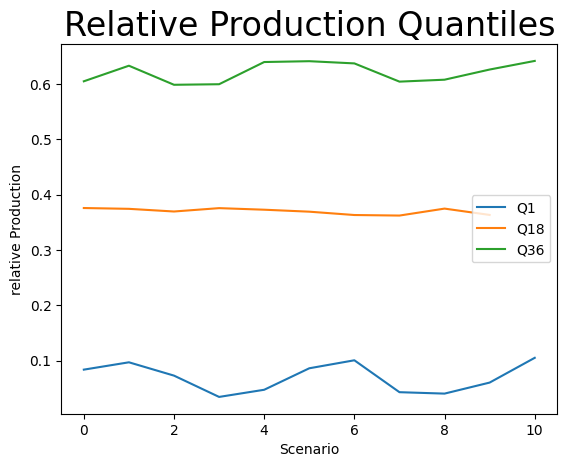
\includegraphics[width=0.7\linewidth]{pictures/results/relativeProduktionQuantils.png}
	\caption{Relative Production Quantiles}
	\label{fig:Relative Production Quantiles}
\end{figure}

Die daraus Resultierenden Zeitreihen für aktivierte Regelarbeit und deren Preise stellen sich dann wie folgt dar:

Für den selben Zeitabschnitt lässt sich der DA Markt wie folgt zusammenfassen:


Außerdem stellt sich der entsprechende RL Markt wie folgt dar:

Dabei zeigt sich das mit steigender Marktdurchdringung der volatilen Energieproduktionsquellen vor allem die Menge an aktivierter Negativer
RegelArbeit steigt während die nachfrage nach positiver regelarbeit fällt.

Ein ähnliches Bild zeigt sich bei den Grenzpreisen für die aktivierte Regelarbeit. wärend die Preise für negative Regelarbeit mit
zunehmenden Anteil an volatilen Produzenten zunimmt, gehen die Preise für die positive Regelarbeit zurück.

Bemerkenswert ist allerdings das sehr hohe Ausreißer in den Zeitreihen für die Grenzpreise der  positiven Regelarbeit bei mittlere und geringer
Marktdurchdringung durch volatile Produzenten zu sehen ist.
--> das liegt vermutlich daran das in den Szenarien wo man mögliche große schwankungen erwartet darauf vorbeiretet ist.
--> Aber in den Szenarien in denen die mehrheit der Anbieter nicht damit rechnet scheint eine unerwartet hohe Nachfrage
--> einen preisschock aus zu lösen.

Die medianen \todo{eventuell nochmal erklärung in data abschnitt wieso das hier die medianen sind} KApazitätspreise für Regelarbeit peaken
sowohl für die negative als auch für die positive im mittleren Szenario. In den Daten des ersten Quantils sind die sie für die negative Regelleistung
vergleichbar mit denen des 36. Quantils. Für die positive Regelleistung hebt sich das 36. Quantil von 1. Quantil vor allem im späten Tagesverlauf ab.

--> es scheint so als würden viele anbieter damit rechnen am folgenden Tag Regelarbeit zu liefern. Dabei hantiert der Regelleistungspreis
--> als eine Art mitnahme preis was zur folge hat das das Angebot noch stärker steigt als die Nachfrage und so sinkende Regelleistungspreise zur folge hat.

Auf Grundlage dieser Zeitreihen hat das Model folgende Daten ermittelt.

Die Strategie für die Gebotspreise für den Kapazitätsmarkt bewegt sich über alle Szenarien hinweg knapp unterhalb des erwarteten Grenzpreises.
\todo{grafik hierfür einblenden  .. !! eher wichtig !!}

Zu sehen ist das die Bereitstellung der negativen RegelArbeit
in den niedrigen und mittleren Szenarien früher erfolgt wenn beide Regelleistungsgebot angenommen wurden [Figure \ref{fig:Negative Balance Energy - Q1}, \ref{fig:Negative Balance Energy - Q18}].
--> verpflichtungen und insgesamt regelmäßigere ladekurve wärend in den höheren Preisszenarien mehr wert
--> darauf gelegt wird wirklich die preisspitzen möglichst optimal mit nehmen zu können.
--> ob das in der realität oder perfektes wissen innerhalb des szenarios so erfolgen kann ist fraglich
In den Szenarien mit den hoher produktiver volatilität ist diese Verschiebung nicht fest zu stellen [Figure \ref{fig:Negative Balance Energy - Q36}]


Wärend sich die Gebotsmengen zur postiven Regelarbeit, je nach Bezuschlagung am Regelleistungsmarkt,
kaum in dem niedrigen und mittleren Szenario voneinander unterscheiden. sind deutlichere Unterschiede
im Szenario mit hoher volatiler Produktion zu erkennen. Auch hier erfolgt eine frühere Bereitstellung
der Arbeit bei stärkeren Restriktionen durch die Bezugschlagung am Regelleistungsmarkt.



Zum Verständnis
\begin{enumerate}
	\item Restricted: B $\rightarrow$ accepted RL in \& out
	\item Restricted: O $\rightarrow$ accepted RL out \& declined in
	\item Restricted: I $\rightarrow$ accepted RL in \& declined out
	\item Restricted: N $\rightarrow$ declined RL in \& out
\end{enumerate}

Die Ergebnisse zeigen eine relativ stetiges Gebotsverhalten am Kapazitätsmarkt über alle Szenarien hinweg.

-->Es wird gerade soviel Geboten
das der Batteriespeicher immer sicher die Restriktionen erfüllen kann ohne all zu sehr den Regelarbeitsmarkt zu beeinflussen.

\begin{figure}[!h]
	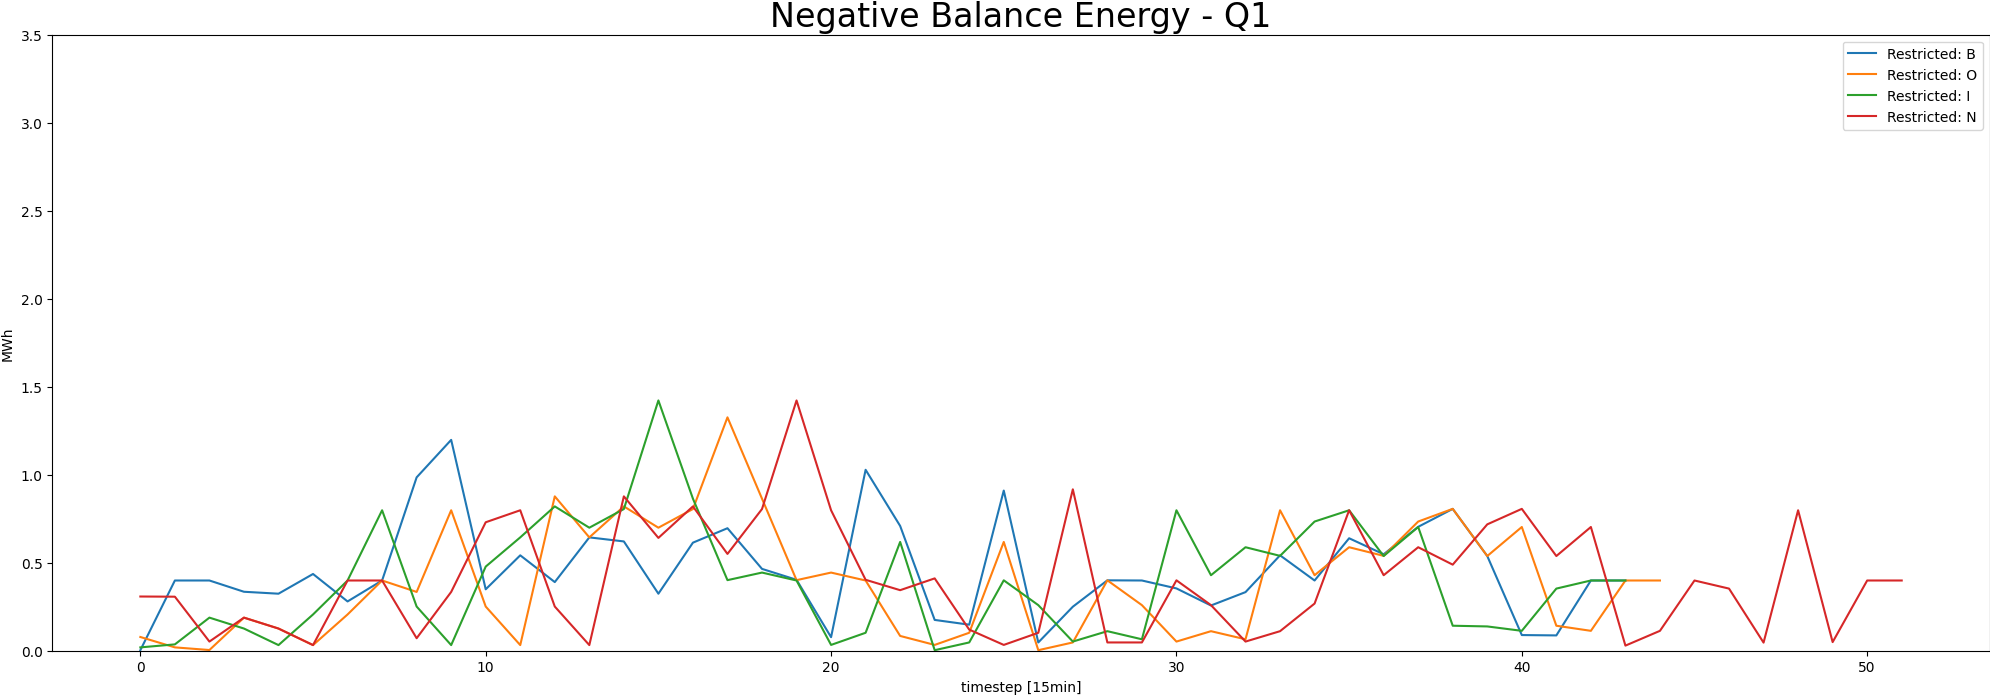
\includegraphics[width=1\linewidth]{pictures/results/Negative Balance Energy - Q1.png}
	\caption{Negative Balance Energy - Q1}
	\label{fig:Negative Balance Energy - Q1}
\end{figure}

\begin{figure}[!h]
	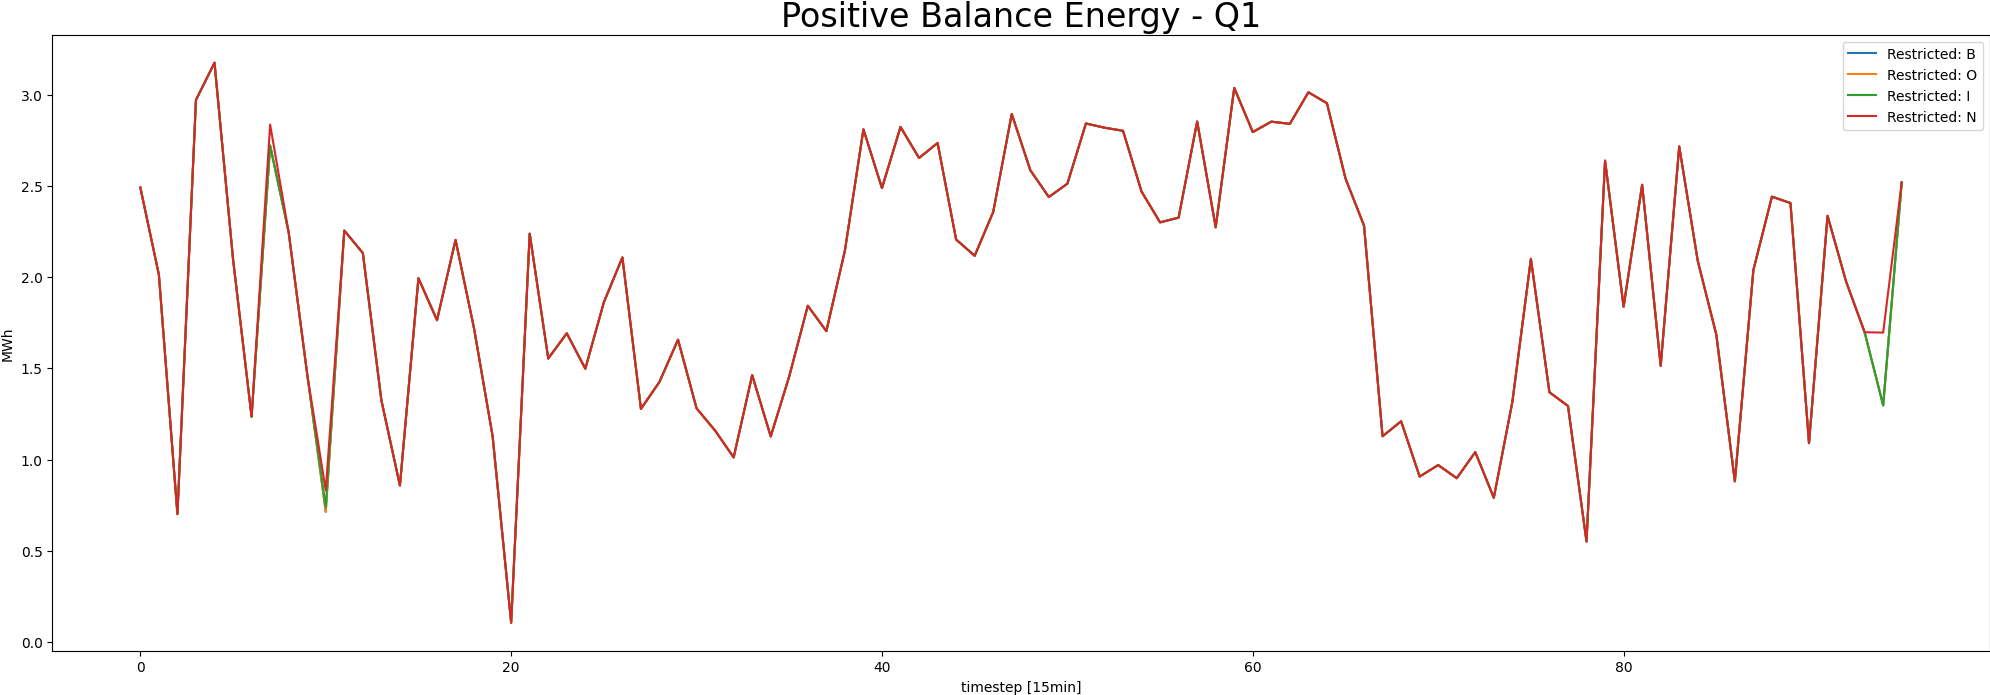
\includegraphics[width=1\linewidth]{pictures/results/Positive Balance Energy - Q1.png}
	\caption{Negative Balance Energy - Q1}
	\label{fig:Negative Balance Energy - Q1}
\end{figure}



\begin{figure}[!h]
	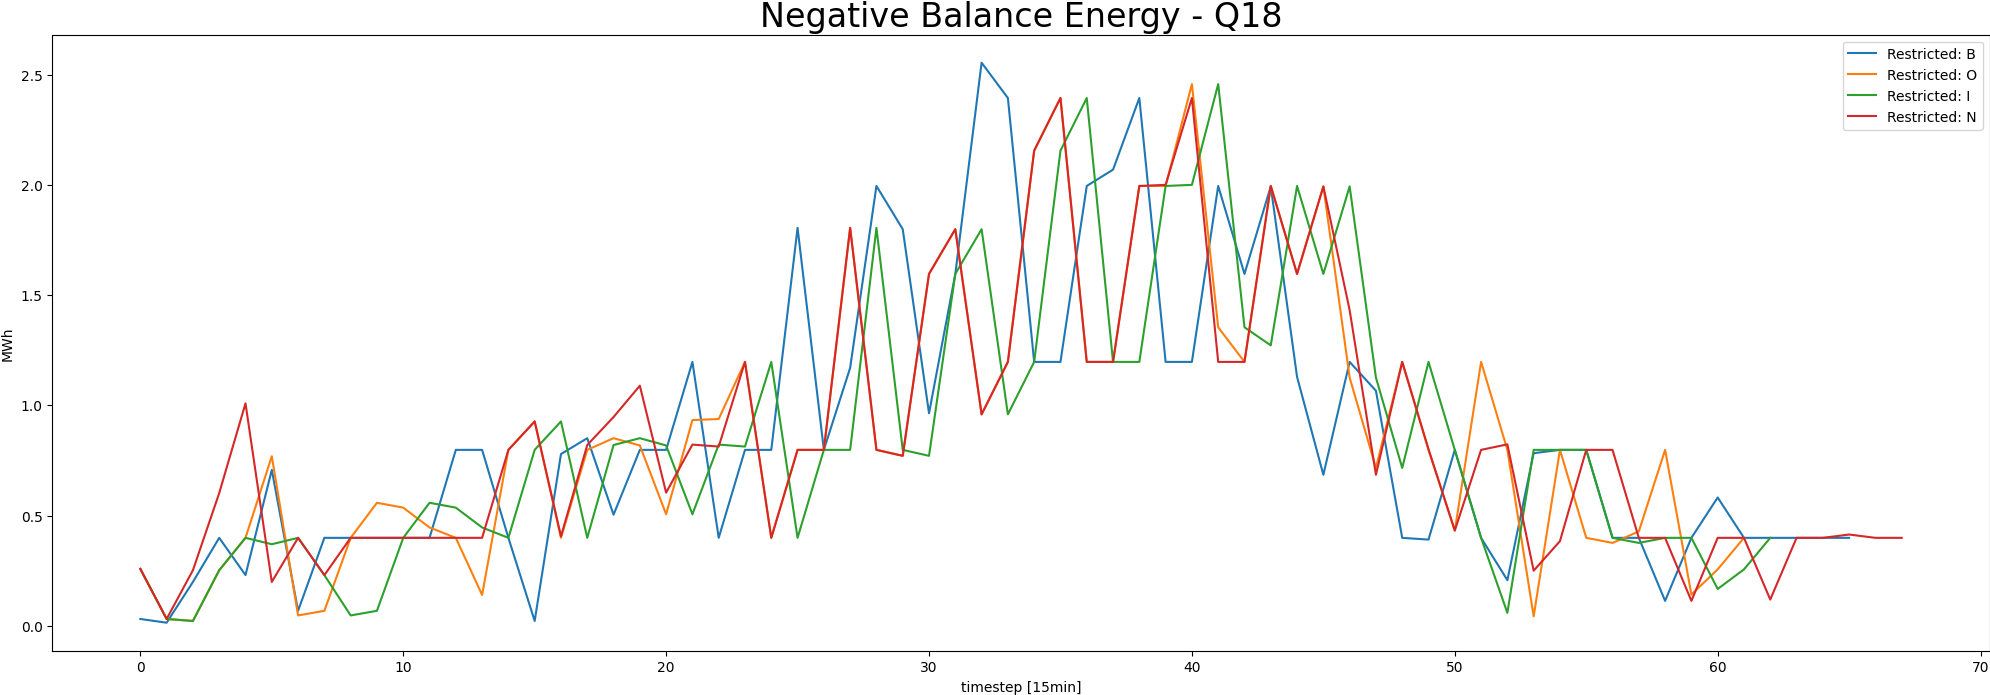
\includegraphics[width=1\linewidth]{pictures/results/Negative Balance Energy - Q18.png}
	\caption{Negative Balance Energy - Q18}
	\label{fig:Negative Balance Energy - Q18}
\end{figure}

\begin{figure}[!h]
	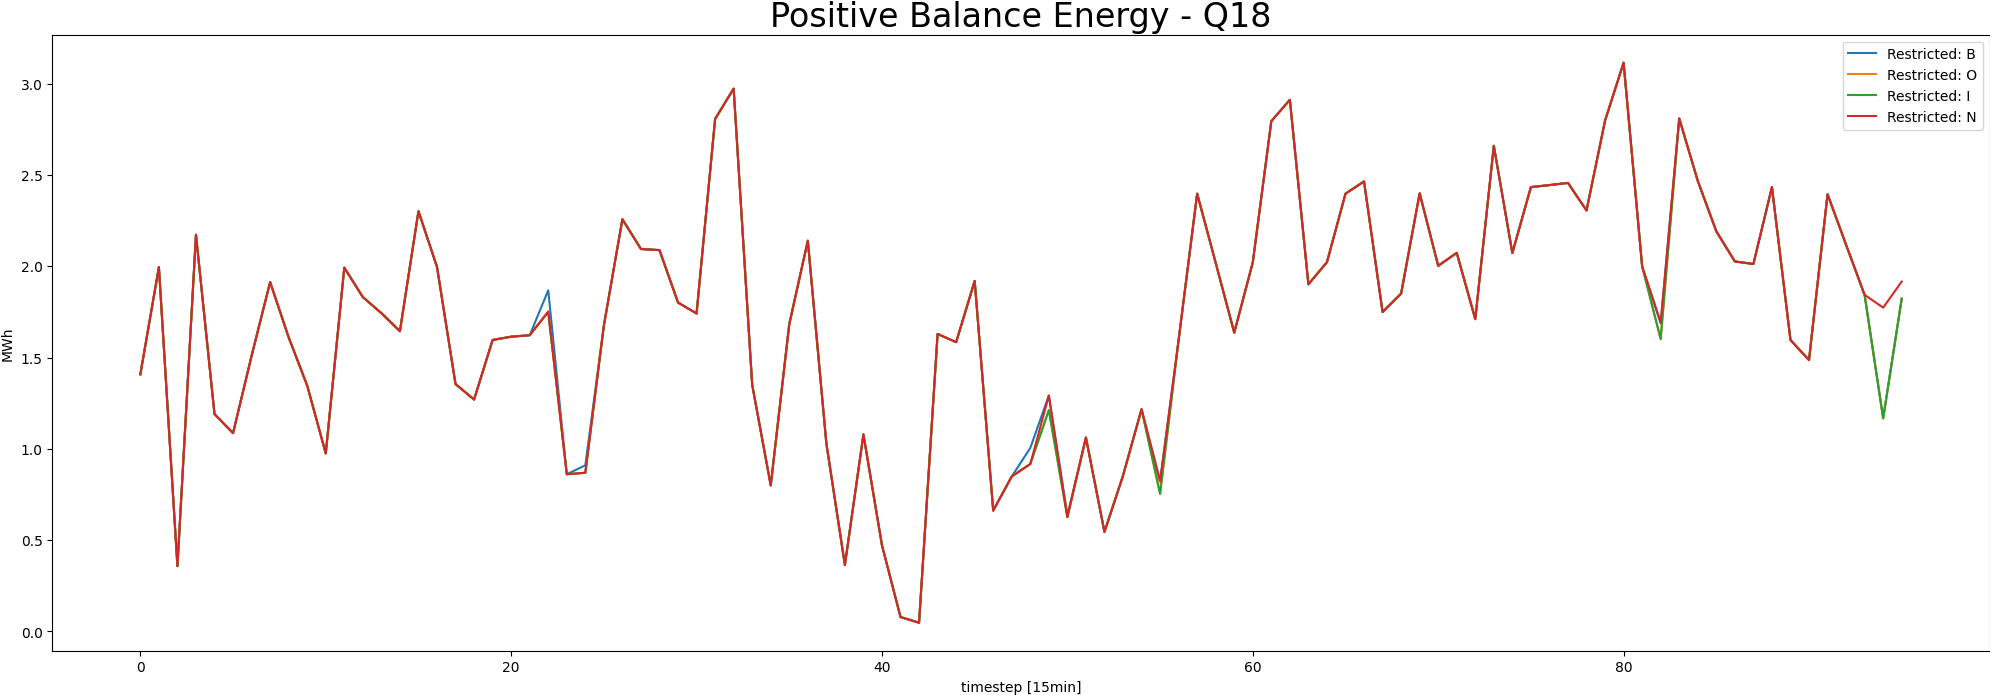
\includegraphics[width=1\linewidth]{pictures/results/Positive Balance Energy - Q18.png}
	\caption{Negative Balance Energy - Q18}
	\label{fig:Negative Balance Energy - Q18}
\end{figure}




\begin{figure}[!h]
	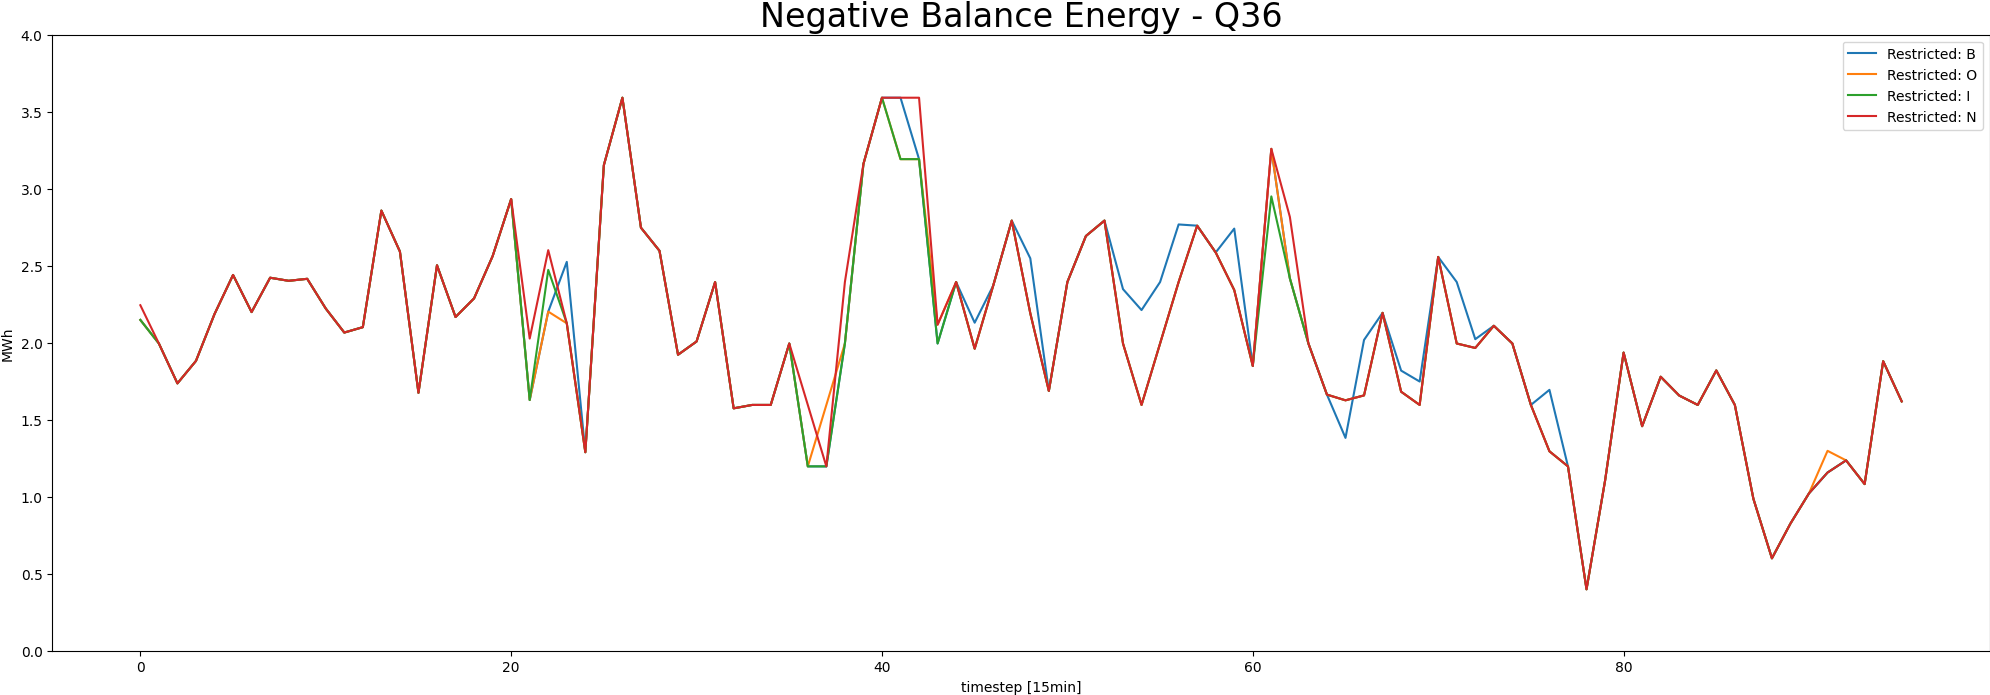
\includegraphics[width=1\linewidth]{pictures/results/Negative Balance Energy - Q36.png}
	\caption{Negative Balance Energy - Q36}
	\label{fig:Negative Balance Energy - Q36}
\end{figure}

\begin{figure}[!h]
	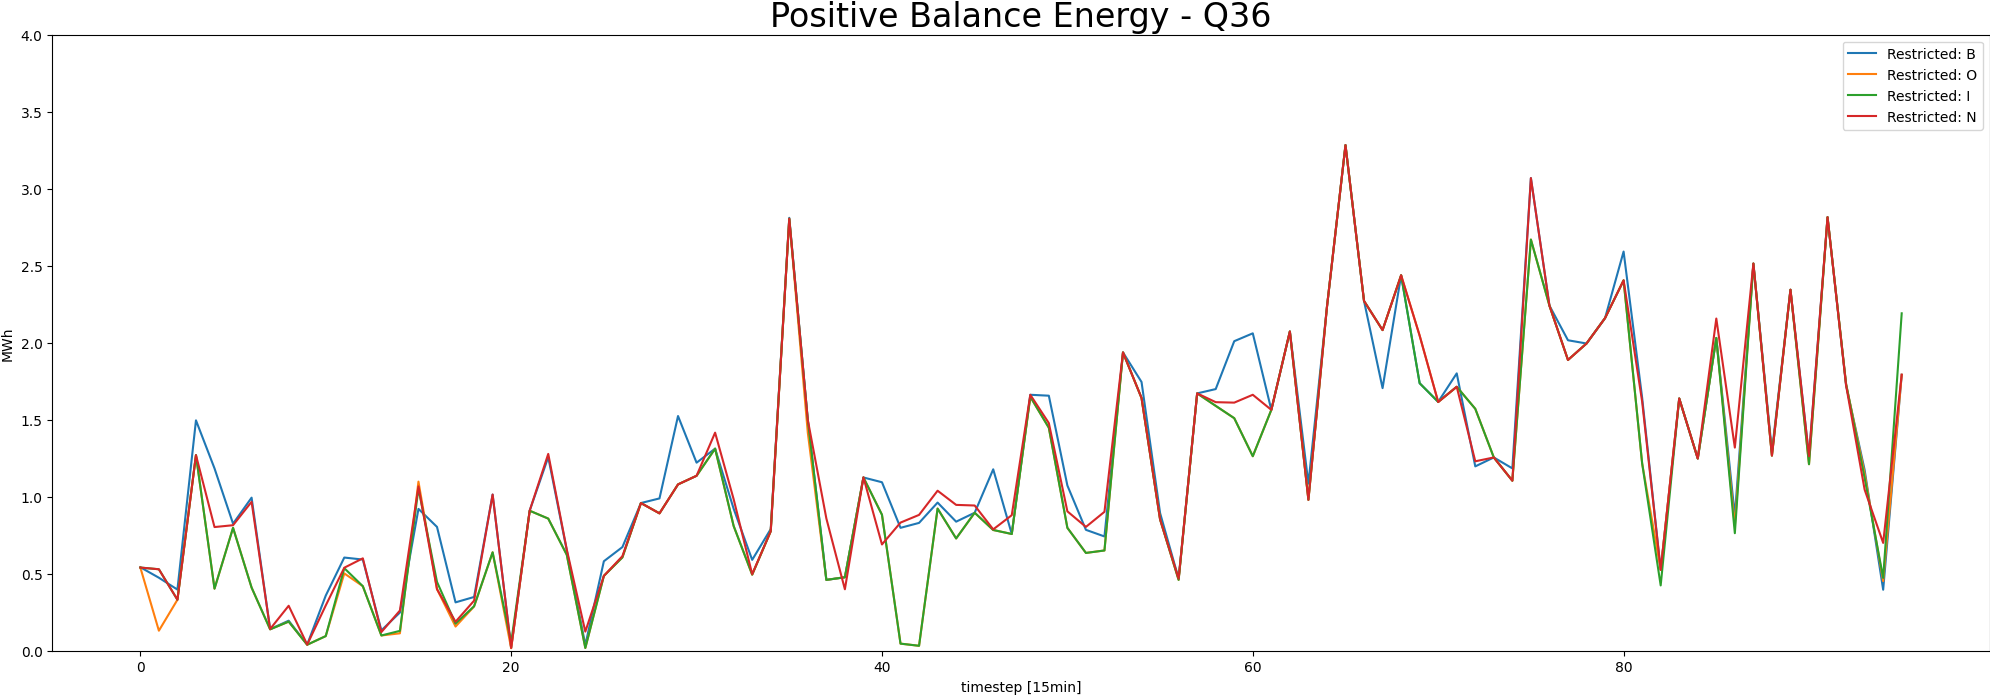
\includegraphics[width=1\linewidth]{pictures/results/Positive Balance Energy - Q36.png}
	\caption{Negative Balance Energy - Q36}
	\label{fig:Negative Balance Energy - Q36}
\end{figure}



\chapter{Conclusion}

Die vorliegenden Analysen zeigen deutlich, dass eine zunehmende Marktdurchdringung durch volatile Energieerzeuger
signifikante Auswirkungen auf die Inanspruchnahme sowie die Preisbildung von Regelarbeit hat.
Insbesondere ist zu beobachten, dass mit steigendem Anteil volatiler Erzeugung die Menge aktivierter negativer Regelarbeit zunimmt,
während gleichzeitig die Nachfrage nach positiver Regelarbeit zurückgeht. Dieses Muster spiegelt sich auch in den Grenzpreisen wider:
Während die Preise für negative Regelarbeit in Abhängigkeit zur Volatilität der Erzeugung steigen, sinken die Preise für positive
Regelarbeit tendenziell.

Auffällig sind zudem starke Preisausreißer bei der positiven Regelarbeit in Szenarien mit geringer oder mittlerer Marktdurchdringung
durch volatile Erzeuger. Diese scheinen auf unerwartet hohe Nachfragespitzen zurückzuführen zu sein, welche in Szenarien auftreten,
in denen Marktteilnehmer nicht mit großen Schwankungen gerechnet haben. Daraus lässt sich schließen, dass die Erwartungshaltung und
Vorbereitung der Marktakteure auf volatile Einspeisung entscheidend zur Preisstabilität beiträgt.

Die analysierten Kapazitätspreise zeigen ein differenziertes Bild: Die Medianwerte peaken sowohl für positive als auch negative
Regelarbeit im mittleren Szenario. Dies deutet auf eine erhöhte Wettbewerbsintensität in diesen Szenarien hin. Gleichzeitig
lässt sich aus den unteren Quantilen ableiten, dass bei negativer Regelarbeit selbst im Vergleich von Q1 zu Q36 kaum Unterschiede
bestehen, während bei positiver Regelarbeit gegen Tagesende eine stärkere Preisdivergenz sichtbar wird. Daraus kann geschlossen werden,
dass Anbieter in Szenarien mit erwarteter hoher volatilät für den Folgetag mit einer Regelarbeitsbereitstellung rechnen und dabei den Kapazitätspreise
als opportunistischen  „Mitnahmepreis“ gestalten. Dies führt dazu, dass das Angebot in Relation zur Nachfrage überproportional
steigt und folglich sinkende Arbeitspreise resultieren.

Die Gebotsstrategien für den Regelleistungsmarkt bewegen sich über alle Szenarien hinweg knapp unterhalb des erwarteten Grenzpreises.

In den Szenarien mit niedriger und mittlere volatiler Producktion zeigt eine verschiebung hin zum negativen Regelleistungsmarkt. Dies zeigt sich
in einem regelmäßigeren Bereitstellung von negativer Regelarbeit. In den Szenarien mit hoher durchdringung und hohen Preisen zeigt sich
am negativen Regelarbeitsmarkt ein Trend möglichst gut die Preisspitzen mitnehmen zu können, dafür wird auf Profit am Regelleistungsmarkt
verzichtet.




Besonders im Bereich negativer Regelarbeit  ist zu erkennen, dass die Bereitstellung in Szenarien mit niedrigem und mittlerem Preisniveau
tendenziell früher erfolgt.  Dies lässt auf eine stärkere Bindung an Verpflichtungen und eine regelmäßigere Ladeplanung schließen.
In höheren Preisszenarien hingegen liegt der Fokus stärker auf einer optimalen Ausnutzung der Preisspitzen - ein Verhalten, das unter realen Marktbedingungen
nicht zwingend replizierbar ist, da es perfektes Wissen über zukünftige Preispfade voraussetzt.

Die Analyse positiver Regelarbeit verdeutlicht hingegen, dass sich Gebotsmengen in niedrig- und mittelfrequentierten Szenarien
nur geringfügig unterscheiden. Erst bei hoher Einspeisung volatiler Energien treten deutliche Unterschiede auf. Auch hier zeigt
sich: Je stärker die Restriktionen durch die Bezuschlagung im Regelleistungsmarkt, desto früher erfolgt die Bereitstellung der Regelarbeit.

Insgesamt zeigen die Ergebnisse, dass sowohl die Erwartungshaltung der Marktakteure als auch deren Strategien im Kapazitäts-
und Regelarbeitsmarkt wesentlich zur Preisbildung und zur Systemstabilität beitragen. Eine vertiefte Betrachtung
dieser Wechselwirkungen ist daher auch für regulatorische Überlegungen zur Ausgestaltung künftiger Strommärkte von zentraler Bedeutung.

\begin{enumerate}
	\item nur ein tag, eventuell kommt der richtige reload erst in zusammenhang mit mehreren tagen zum tragen
\end{enumerate}

todo{andere anbieter wirklich mit simulieren}


%% ********************
%% Backmatter
%% ********************
%\backmatter

\chapter{Appendix}
%% change chapter title to german if necessary
%% *** local page settings ***
\markright{Appendix}
\addtocontents{toc}{\protect\setcounter{tocdepth}{-1}} %decrease the depth of the appendix entry in the ToC
\setcounter{table}{0}
\setcounter{figure}{0}
\renewcommand{\thefigure}{A.\arabic{figure}}
\renewcommand{\thetable}{A.\arabic{table}}


\section{Further Model Constraints}

\begin{flalign}
	\label{parkCon_Q^{rB}_{DA}(t_{hour})}                   \sum((s_DA, s^{in}_{RL}, s^{out}_{RL}), Q^{rB}_{DA}(t_{hour}, s^{in}_{RL}, s^{out}_{RL})) \leq parkCap * parkProfile(t_{hour}) - \sum((s_DA, s^{in}_{RL}, s^{out}_{RL}), Q_rB_reload(t_{hour}, s^{in}_{RL}, s^{out}_{RL}));
\end{flalign}
\begin{flalign}
	\label{parkCon_Q^{rI}_{DA}(t_{hour})}                   \sum((s_DA, s^{in}_{RL}, s^{out}_{RL}), Q^{rI}_{DA}(t_{hour}, s^{in}_{RL}, s^{out}_{RL})) \leq parkCap * parkProfile(t_{hour}) - \sum((s_DA, s^{in}_{RL}, s^{out}_{RL}), Q_rI_reload(t_{hour}, s^{in}_{RL}, s^{out}_{RL}));
\end{flalign}
\begin{flalign}
	\label{parkCon_Q^{rO}_{DA}(t_{hour})}                   \sum((s_DA, s^{in}_{RL}, s^{out}_{RL}), Q^{rO}_{DA}(t_{hour}, s^{in}_{RL}, s^{out}_{RL})) \leq parkCap * parkProfile(t_{hour}) - \sum((s_DA, s^{in}_{RL}, s^{out}_{RL}), Q_rO_reload(t_{hour}, s^{in}_{RL}, s^{out}_{RL}));
\end{flalign}
\begin{flalign}
	\label{parkCon_Q^{rN}_{DA}(t_{hour})}                   \sum((s_DA, s^{in}_{RL}, s^{out}_{RL}), Q^{rN}_{DA}(t_{hour}, s^{in}_{RL}, s^{out}_{RL})) \leq parkCap * parkProfile(t_{hour}) - \sum((s_DA, s^{in}_{RL}, s^{out}_{RL}), Q_rN_reload(t_{hour}, s^{in}_{RL}, s^{out}_{RL}));
\end{flalign}
\section{Quantile Market Data}

\begin{figure}[!h]
	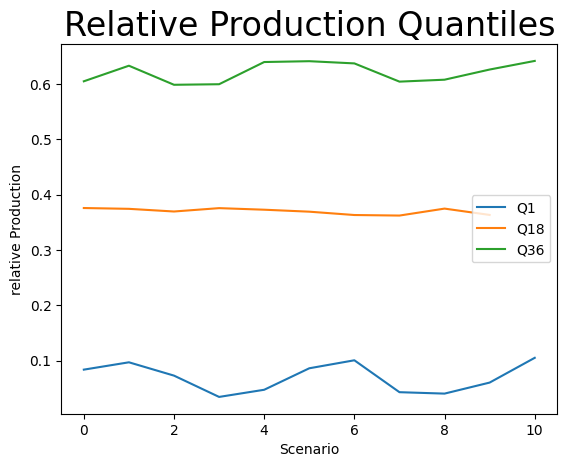
\includegraphics[width=0.7\linewidth]{pictures/results/relativeProduktionQuantils.png}
	\caption{Relative Production Quantiles}
	\label{fig:Relative Production Quantiles}
\end{figure}

Die daraus Resultierenden Zeitreihen für aktivierte Regelarbeit und deren Preise stellen sich dann wie folgt dar:
\begin{figure}[H]
	\centering

	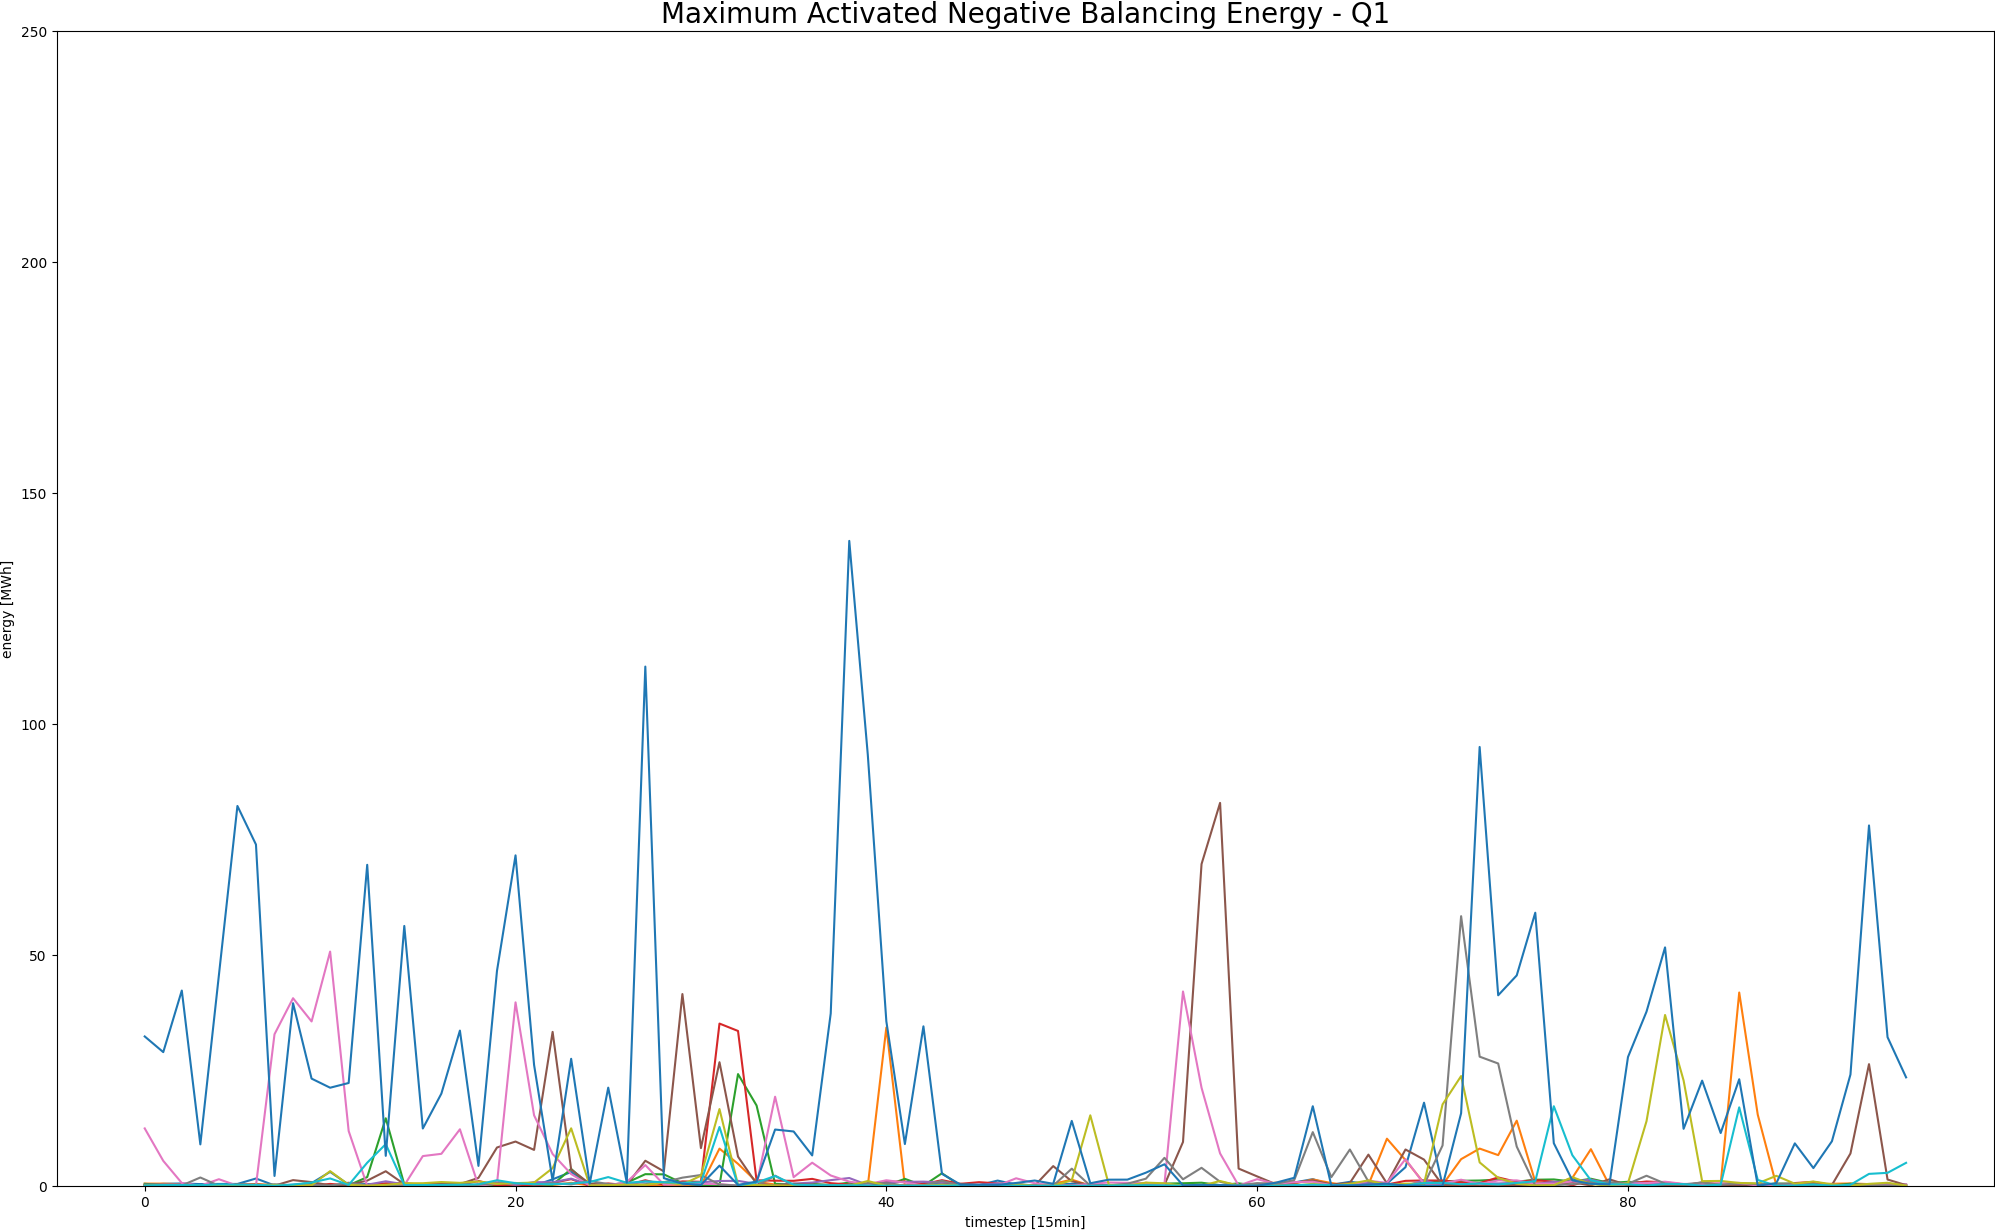
\includegraphics[width=1\linewidth]{pictures/results/Activated_negEnergy_Q1.png}
	\caption{Activated Negative Energy Q1}
	\label{fig:_negEnergy_Q1}
\end{figure}


\begin{figure}[H]
	\centering
	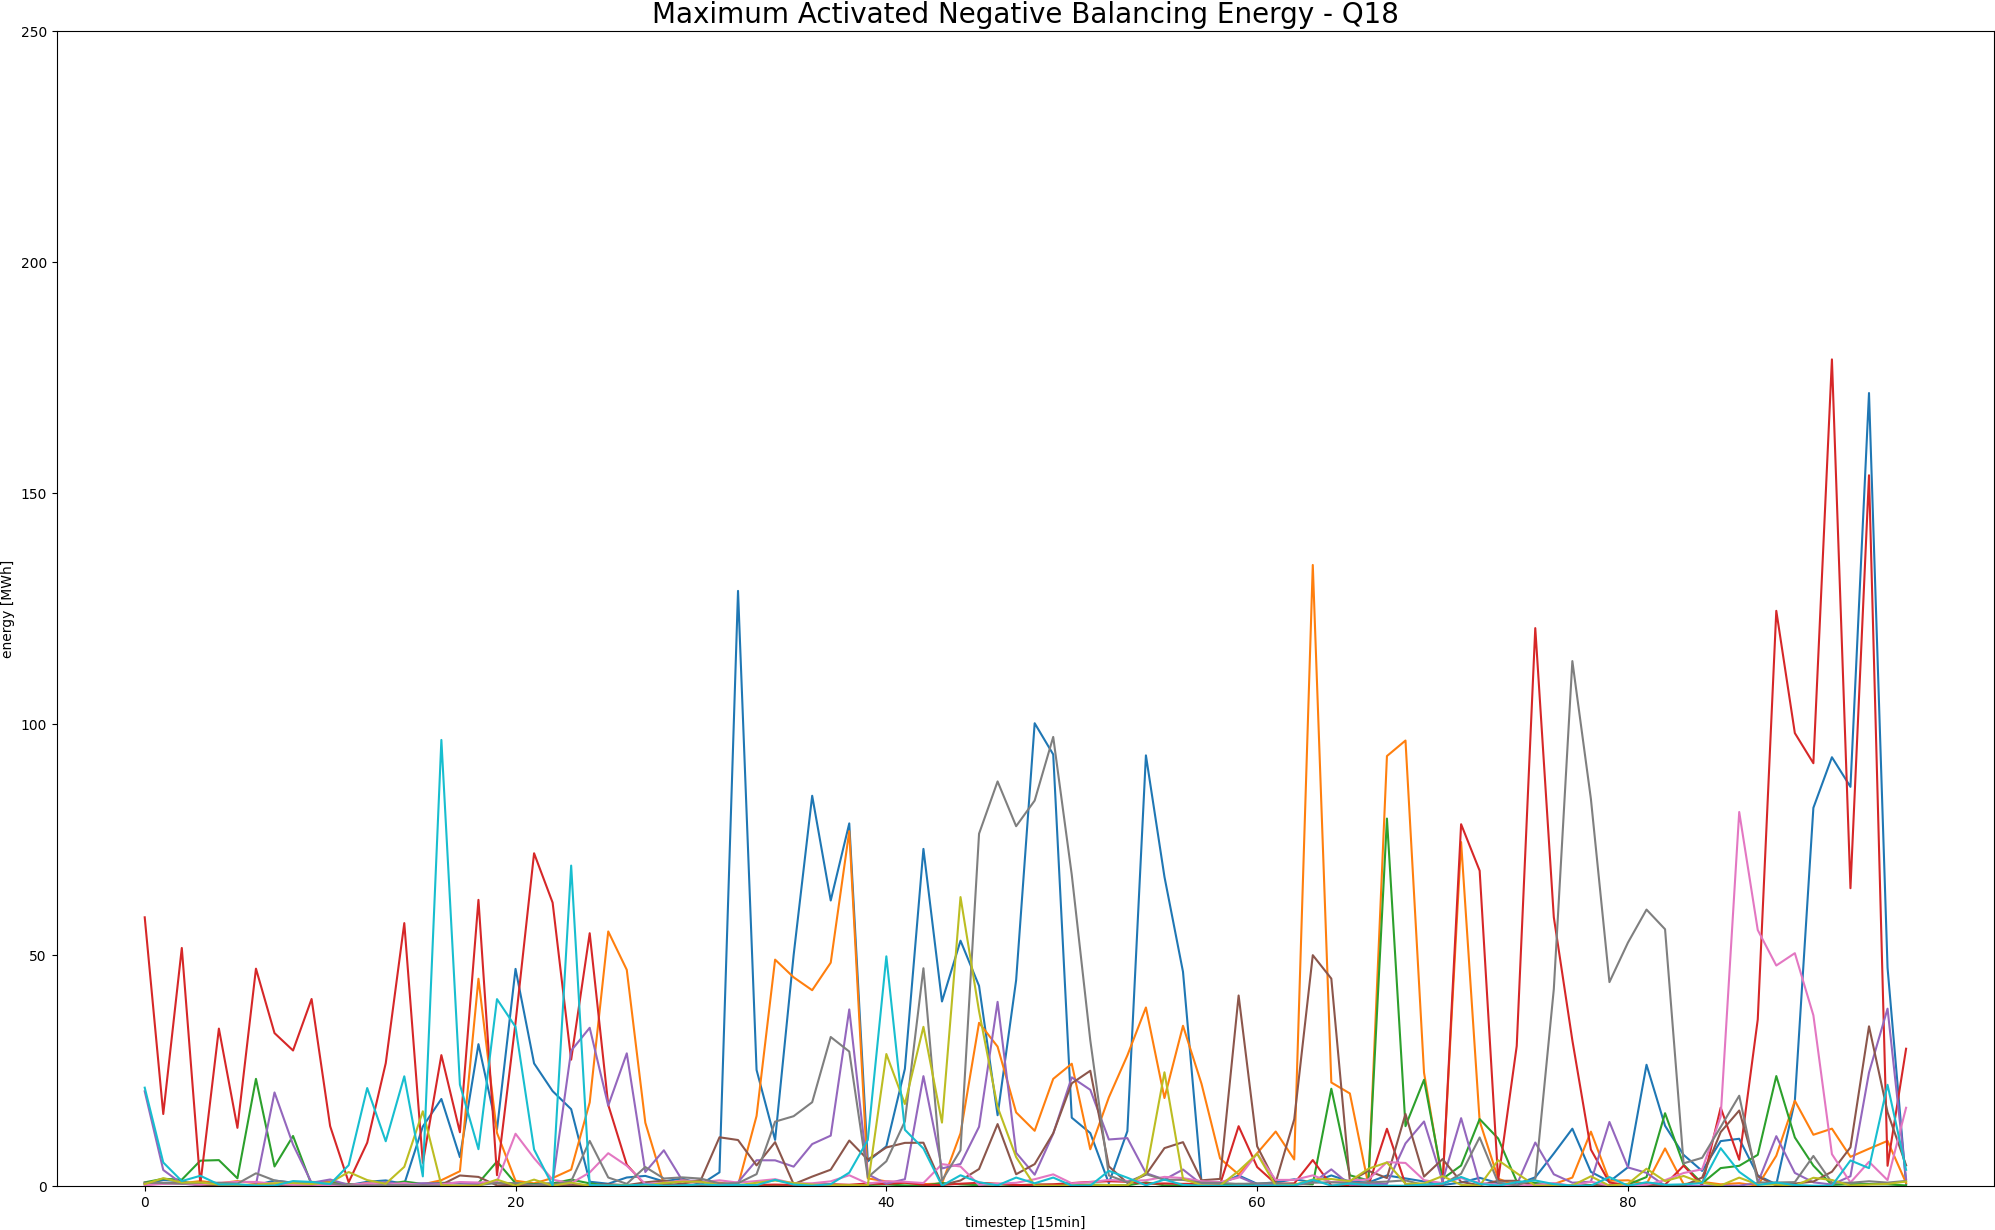
\includegraphics[width=1\linewidth]{pictures/results/Activated_negEnergy_Q18.png}
	\caption{Activated Negative Energy Q18}
	\label{fig:_negEnergy_Q18}
\end{figure}

\begin{figure}[H]
	\centering
	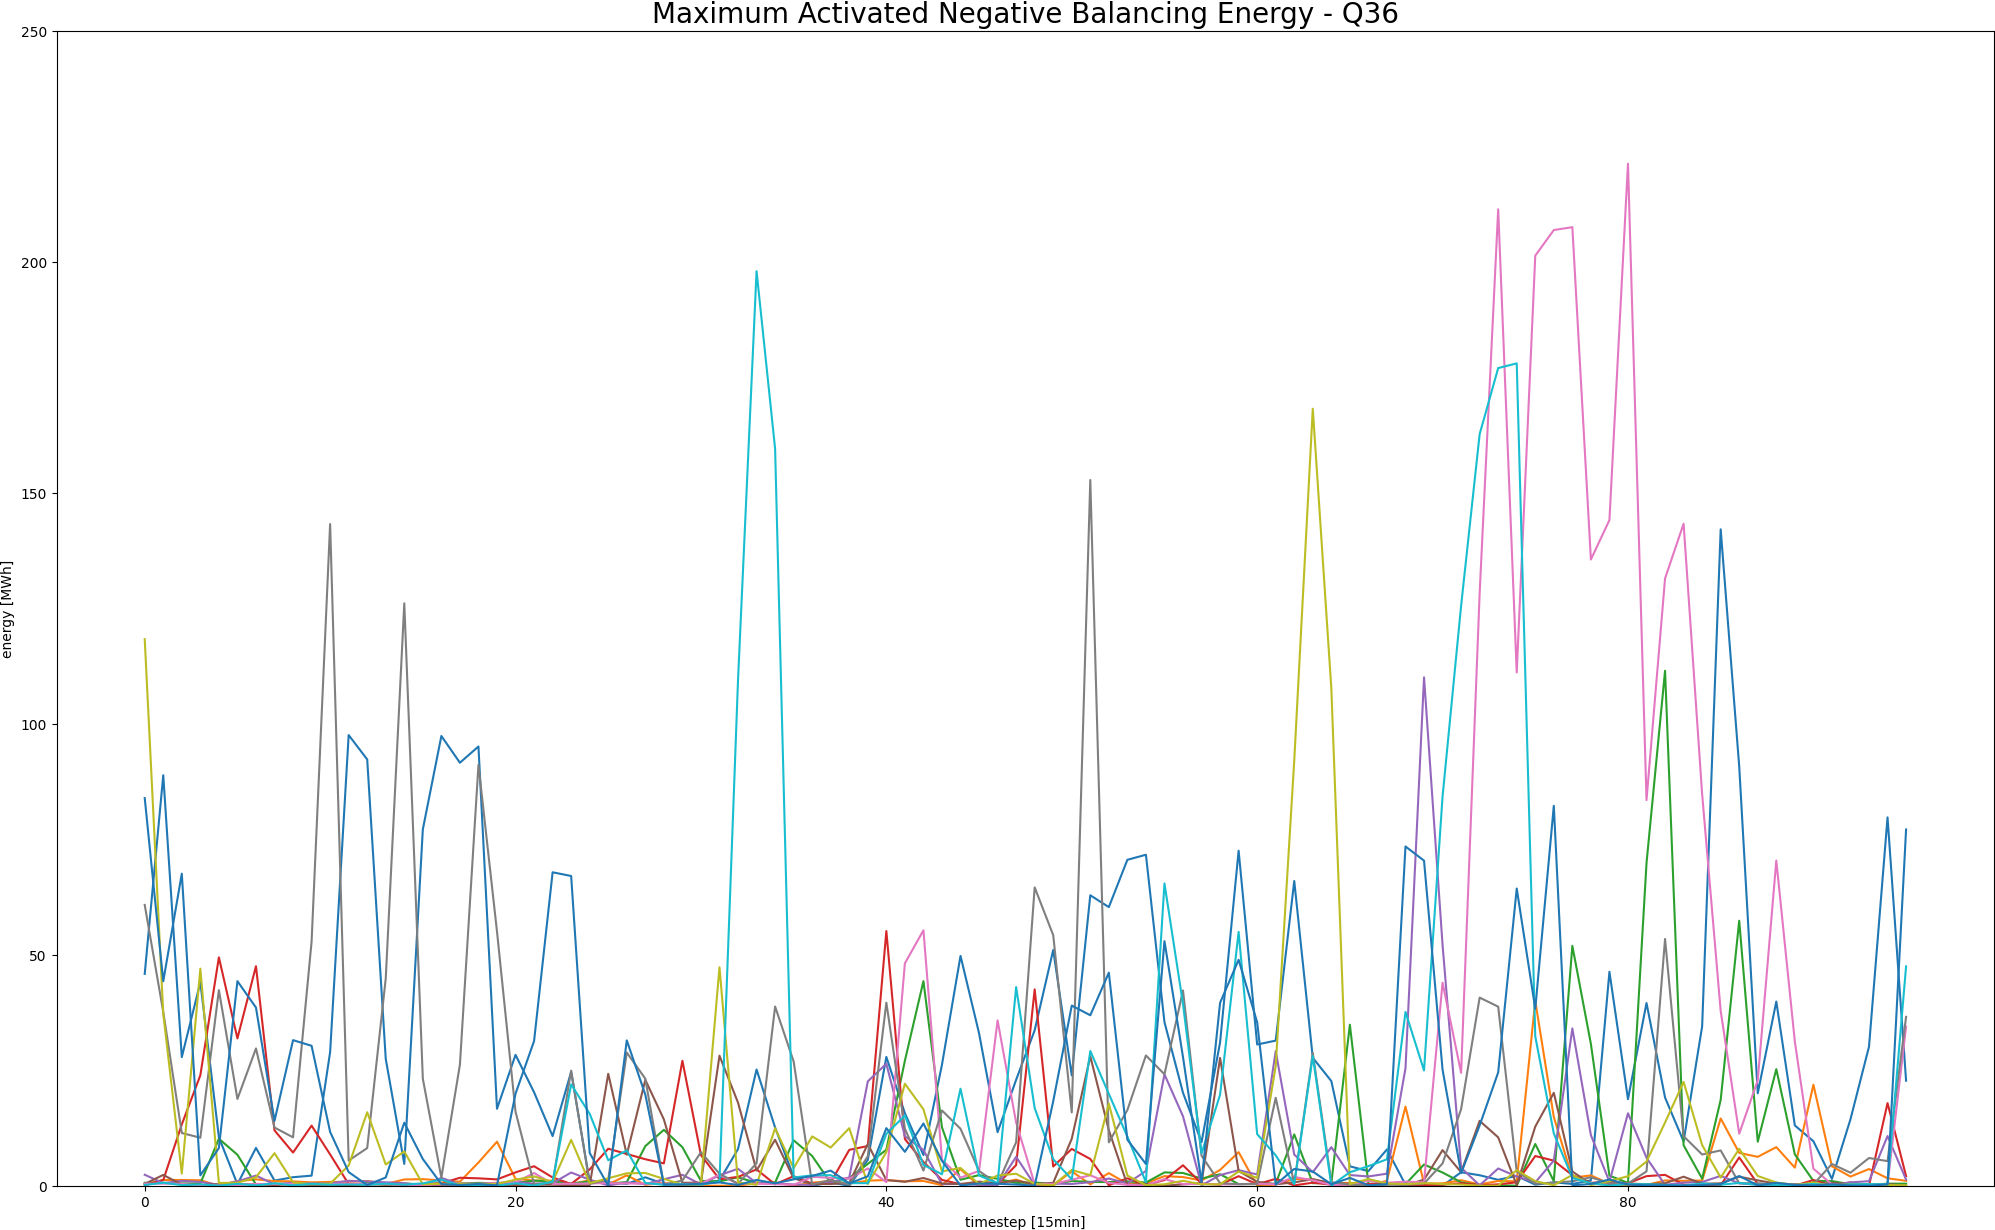
\includegraphics[width=1\linewidth]{pictures/results/Activated_negEnergy_Q36.png}
	\caption{Activated Negative Energy Q36}
	\label{fig:_negEnergy_Q36}
\end{figure}
\begin{figure}
	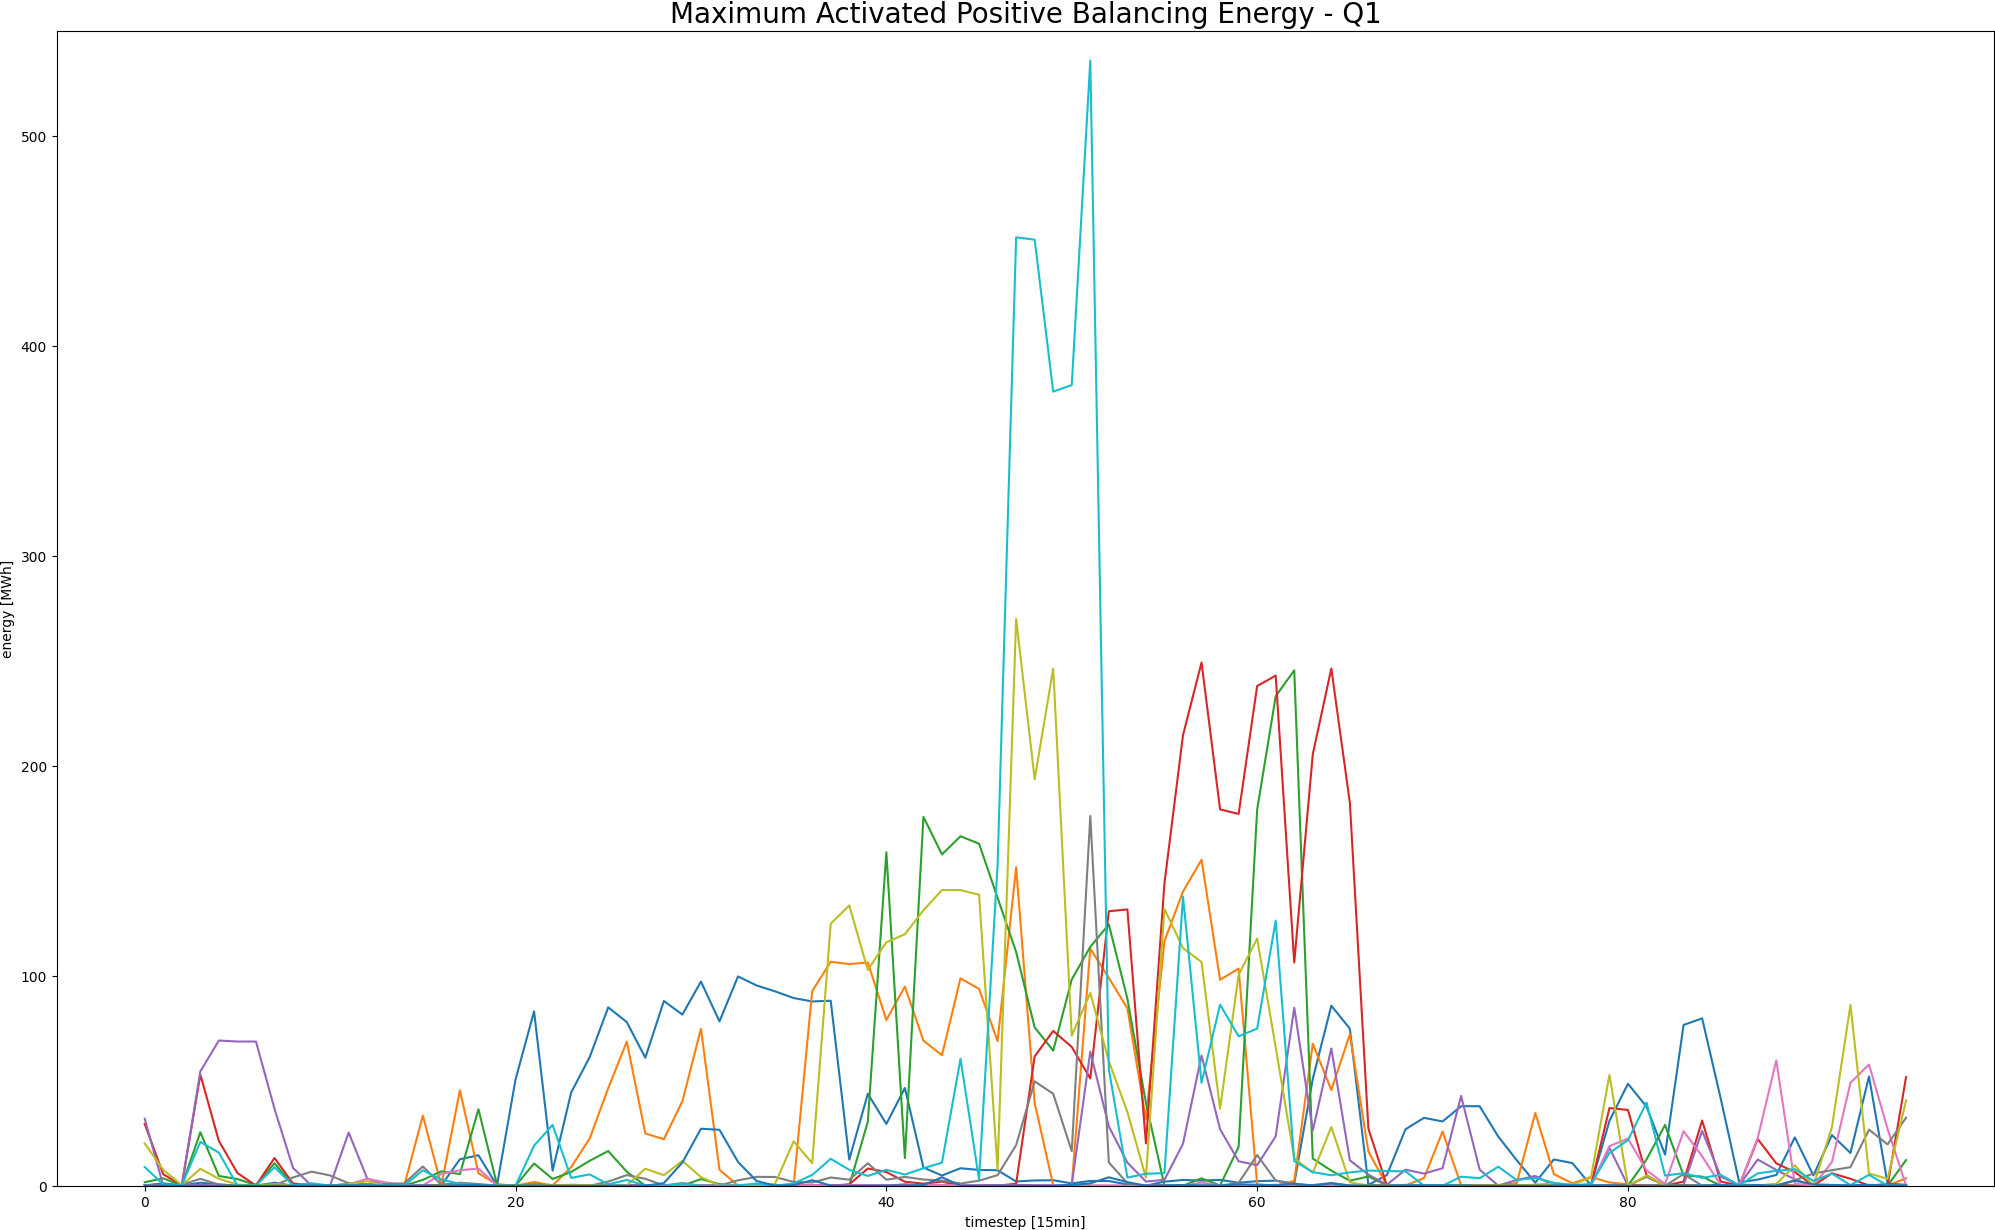
\includegraphics[width=1\linewidth]{pictures/results/Activated_posEnergy_Q1.png}
	\caption{Activated Positive Energy Q1}
	\label{fig:_posEnergy_Q1}
\end{figure}

\begin{figure}
	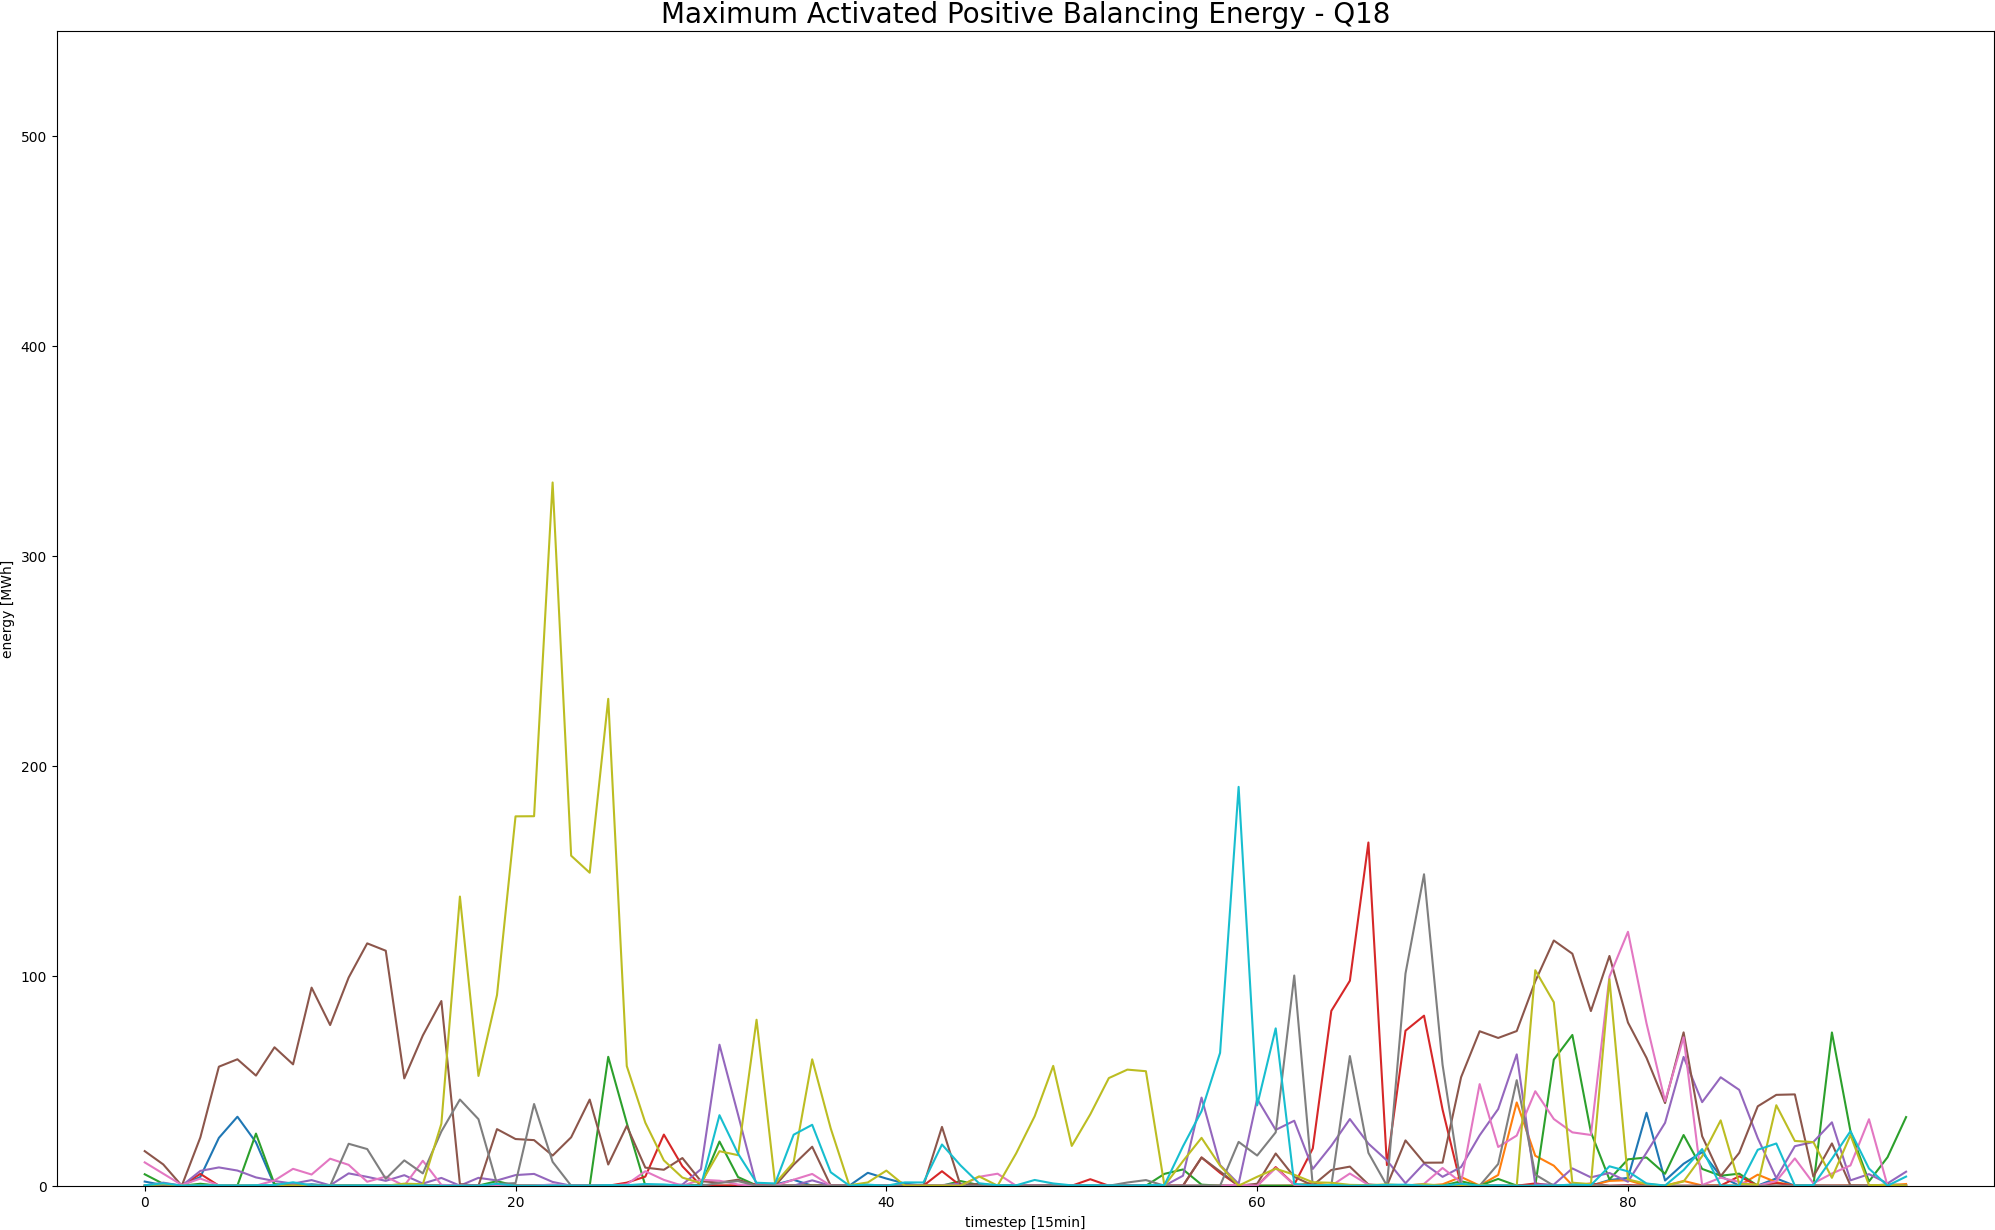
\includegraphics[width=1\linewidth]{pictures/results/Activated_posEnergy_Q18.png}
	\caption{Activated Positive Energy Q18}
	\label{fig:_posEnergy_Q18}
\end{figure}

\begin{figure}
	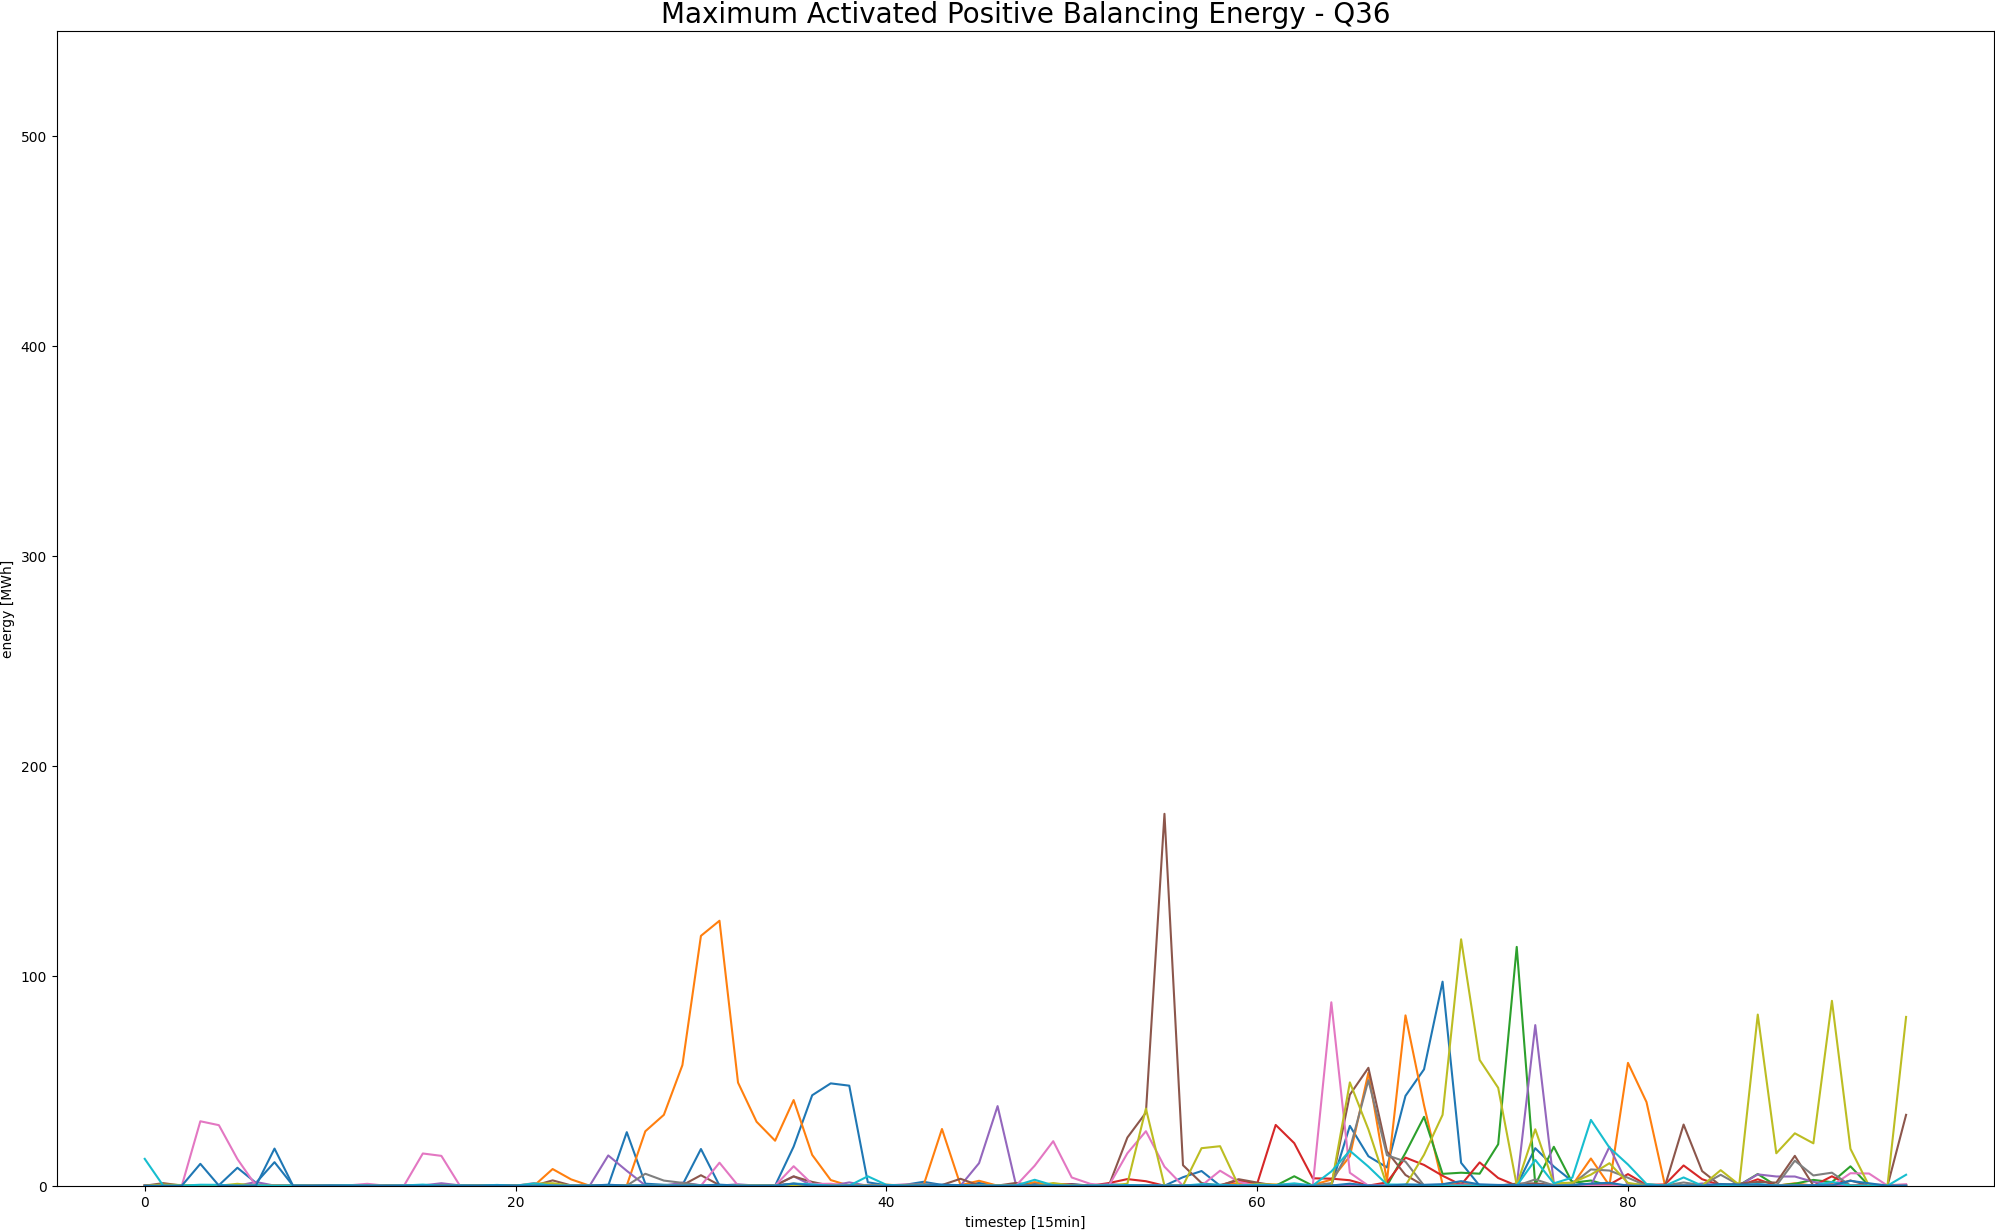
\includegraphics[width=1\linewidth]{pictures/results/Activated_posEnergy_Q36.png}
	\caption{Activated Positive Energy Q36}
	\label{fig:_posEnergy_Q36}
\end{figure}



\begin{figure}[H]
	\centering
	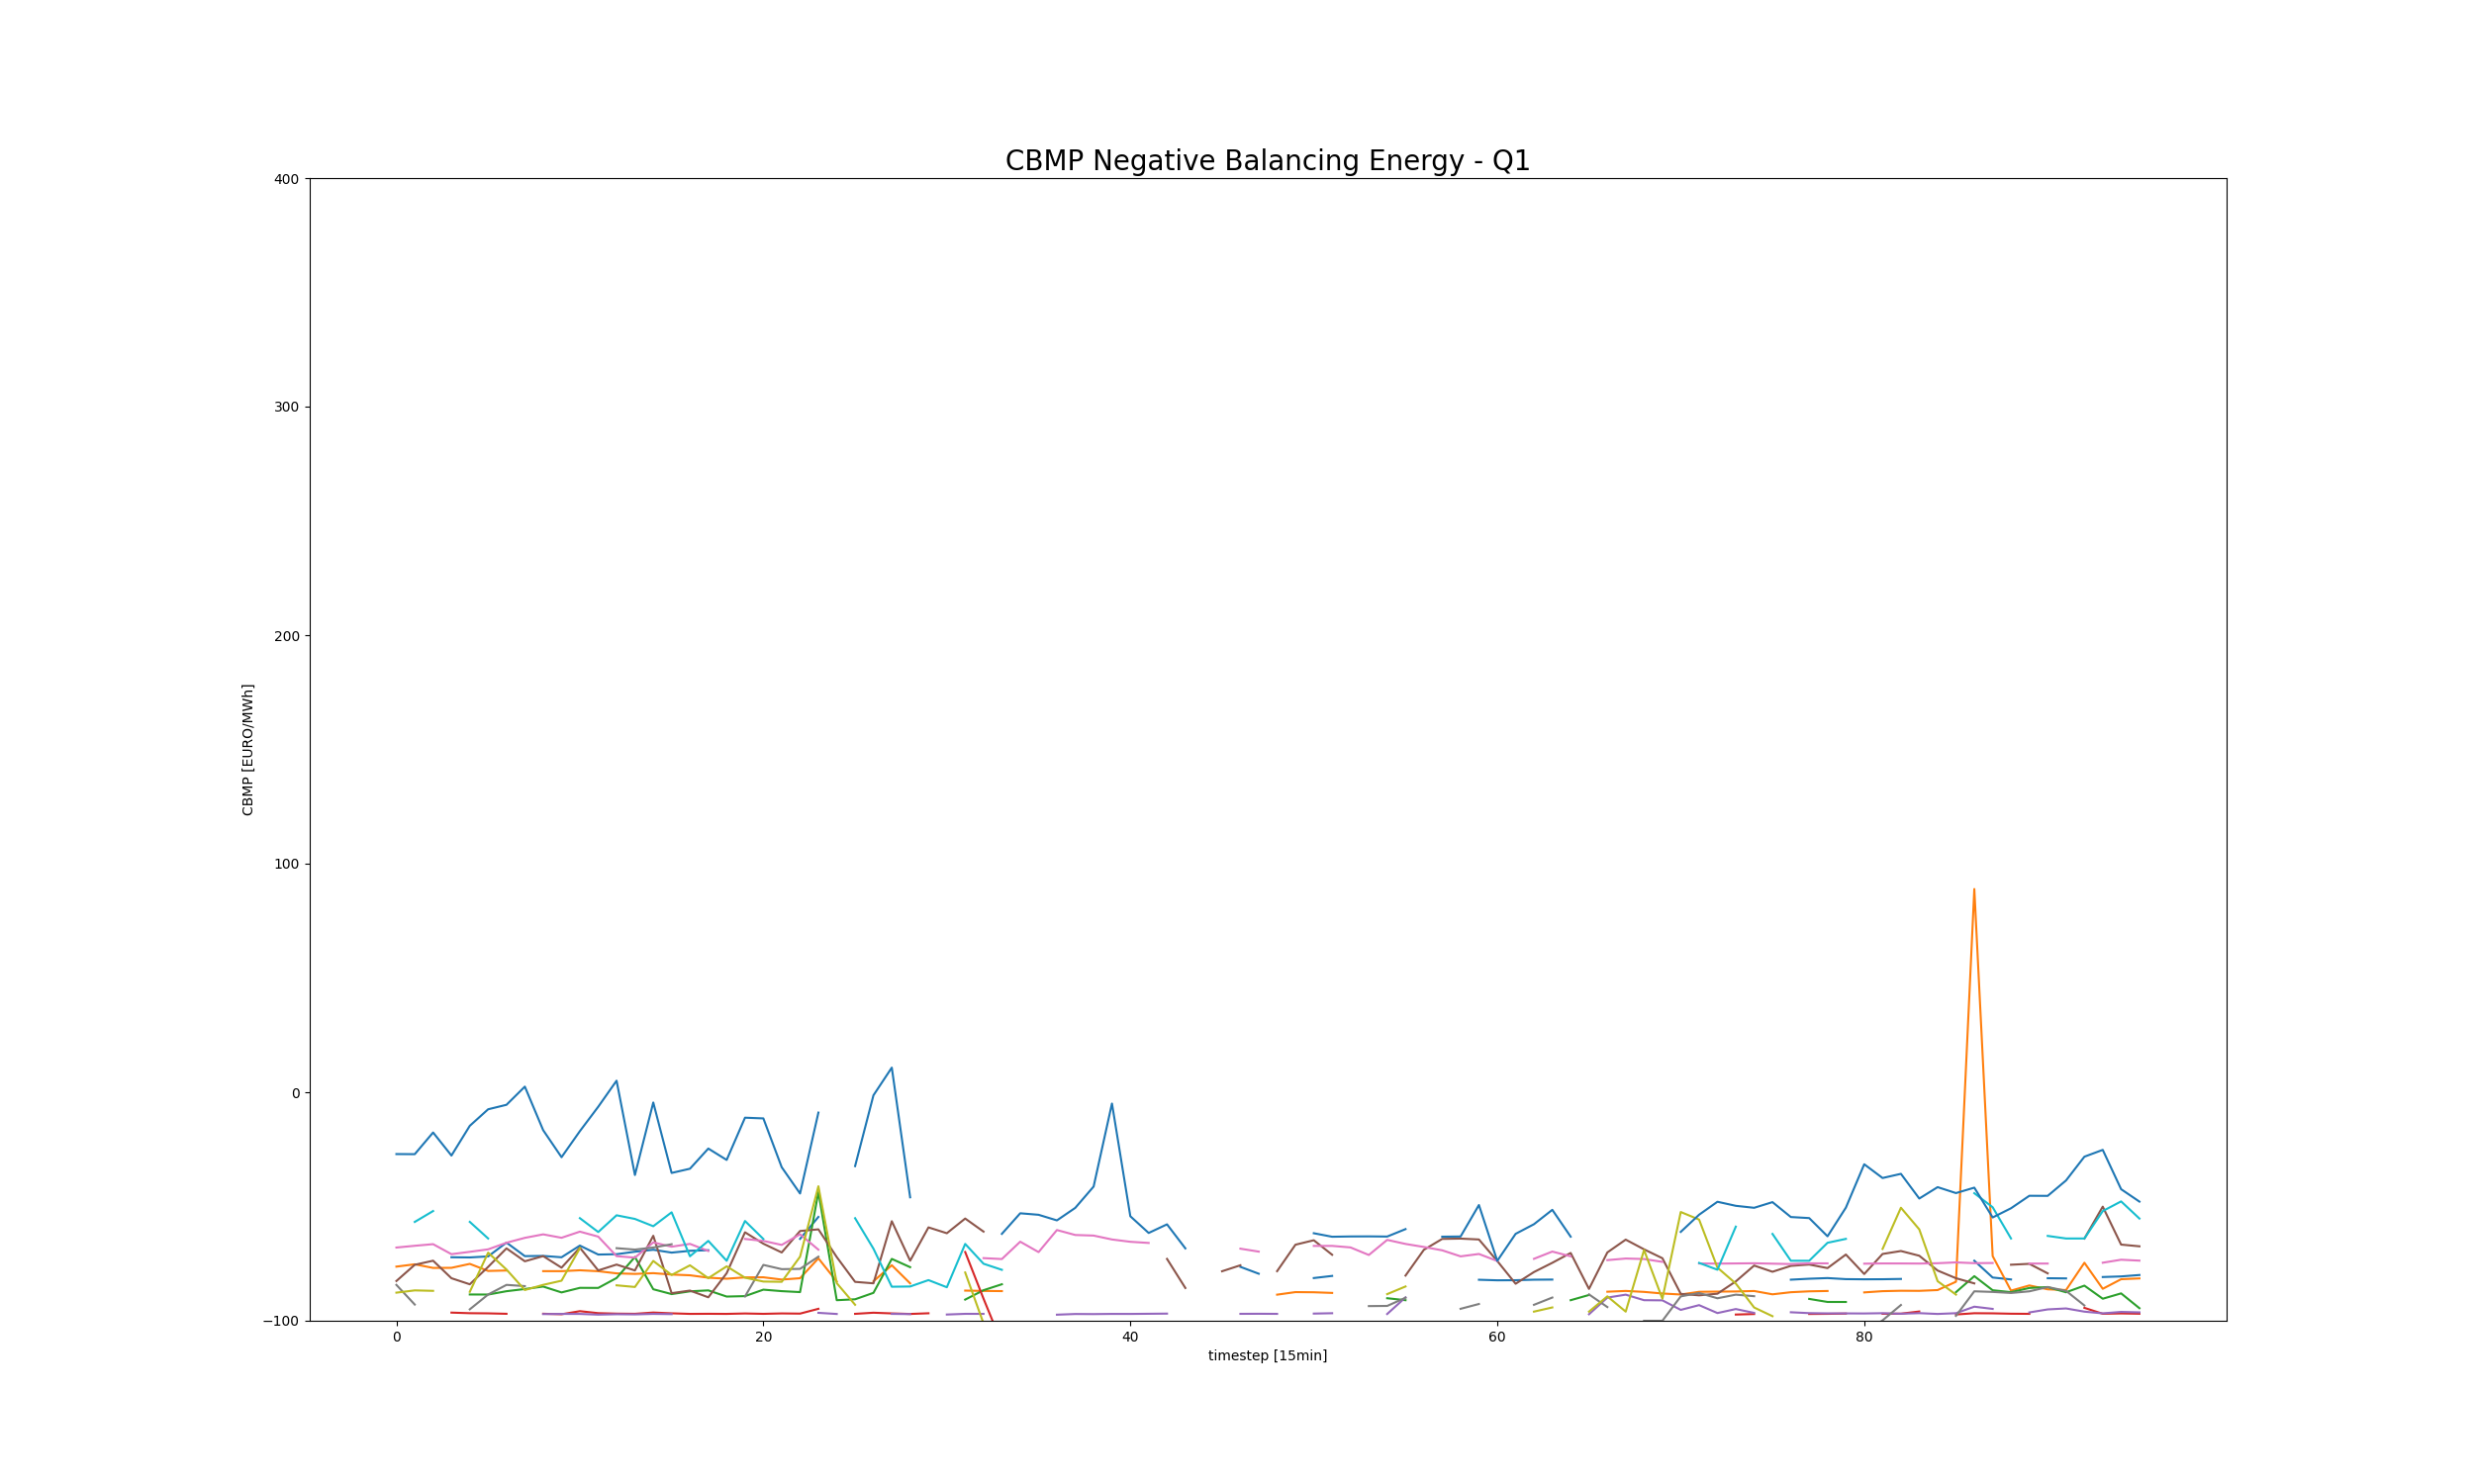
\includegraphics[width=1\linewidth]{pictures/results/CBMP_negBal_Q1.png}
	\caption{CBMP Negative Energy Q1}
	\label{fig:CBMP_negBal_Q1}
\end{figure}


\begin{figure}[H]
	\centering
	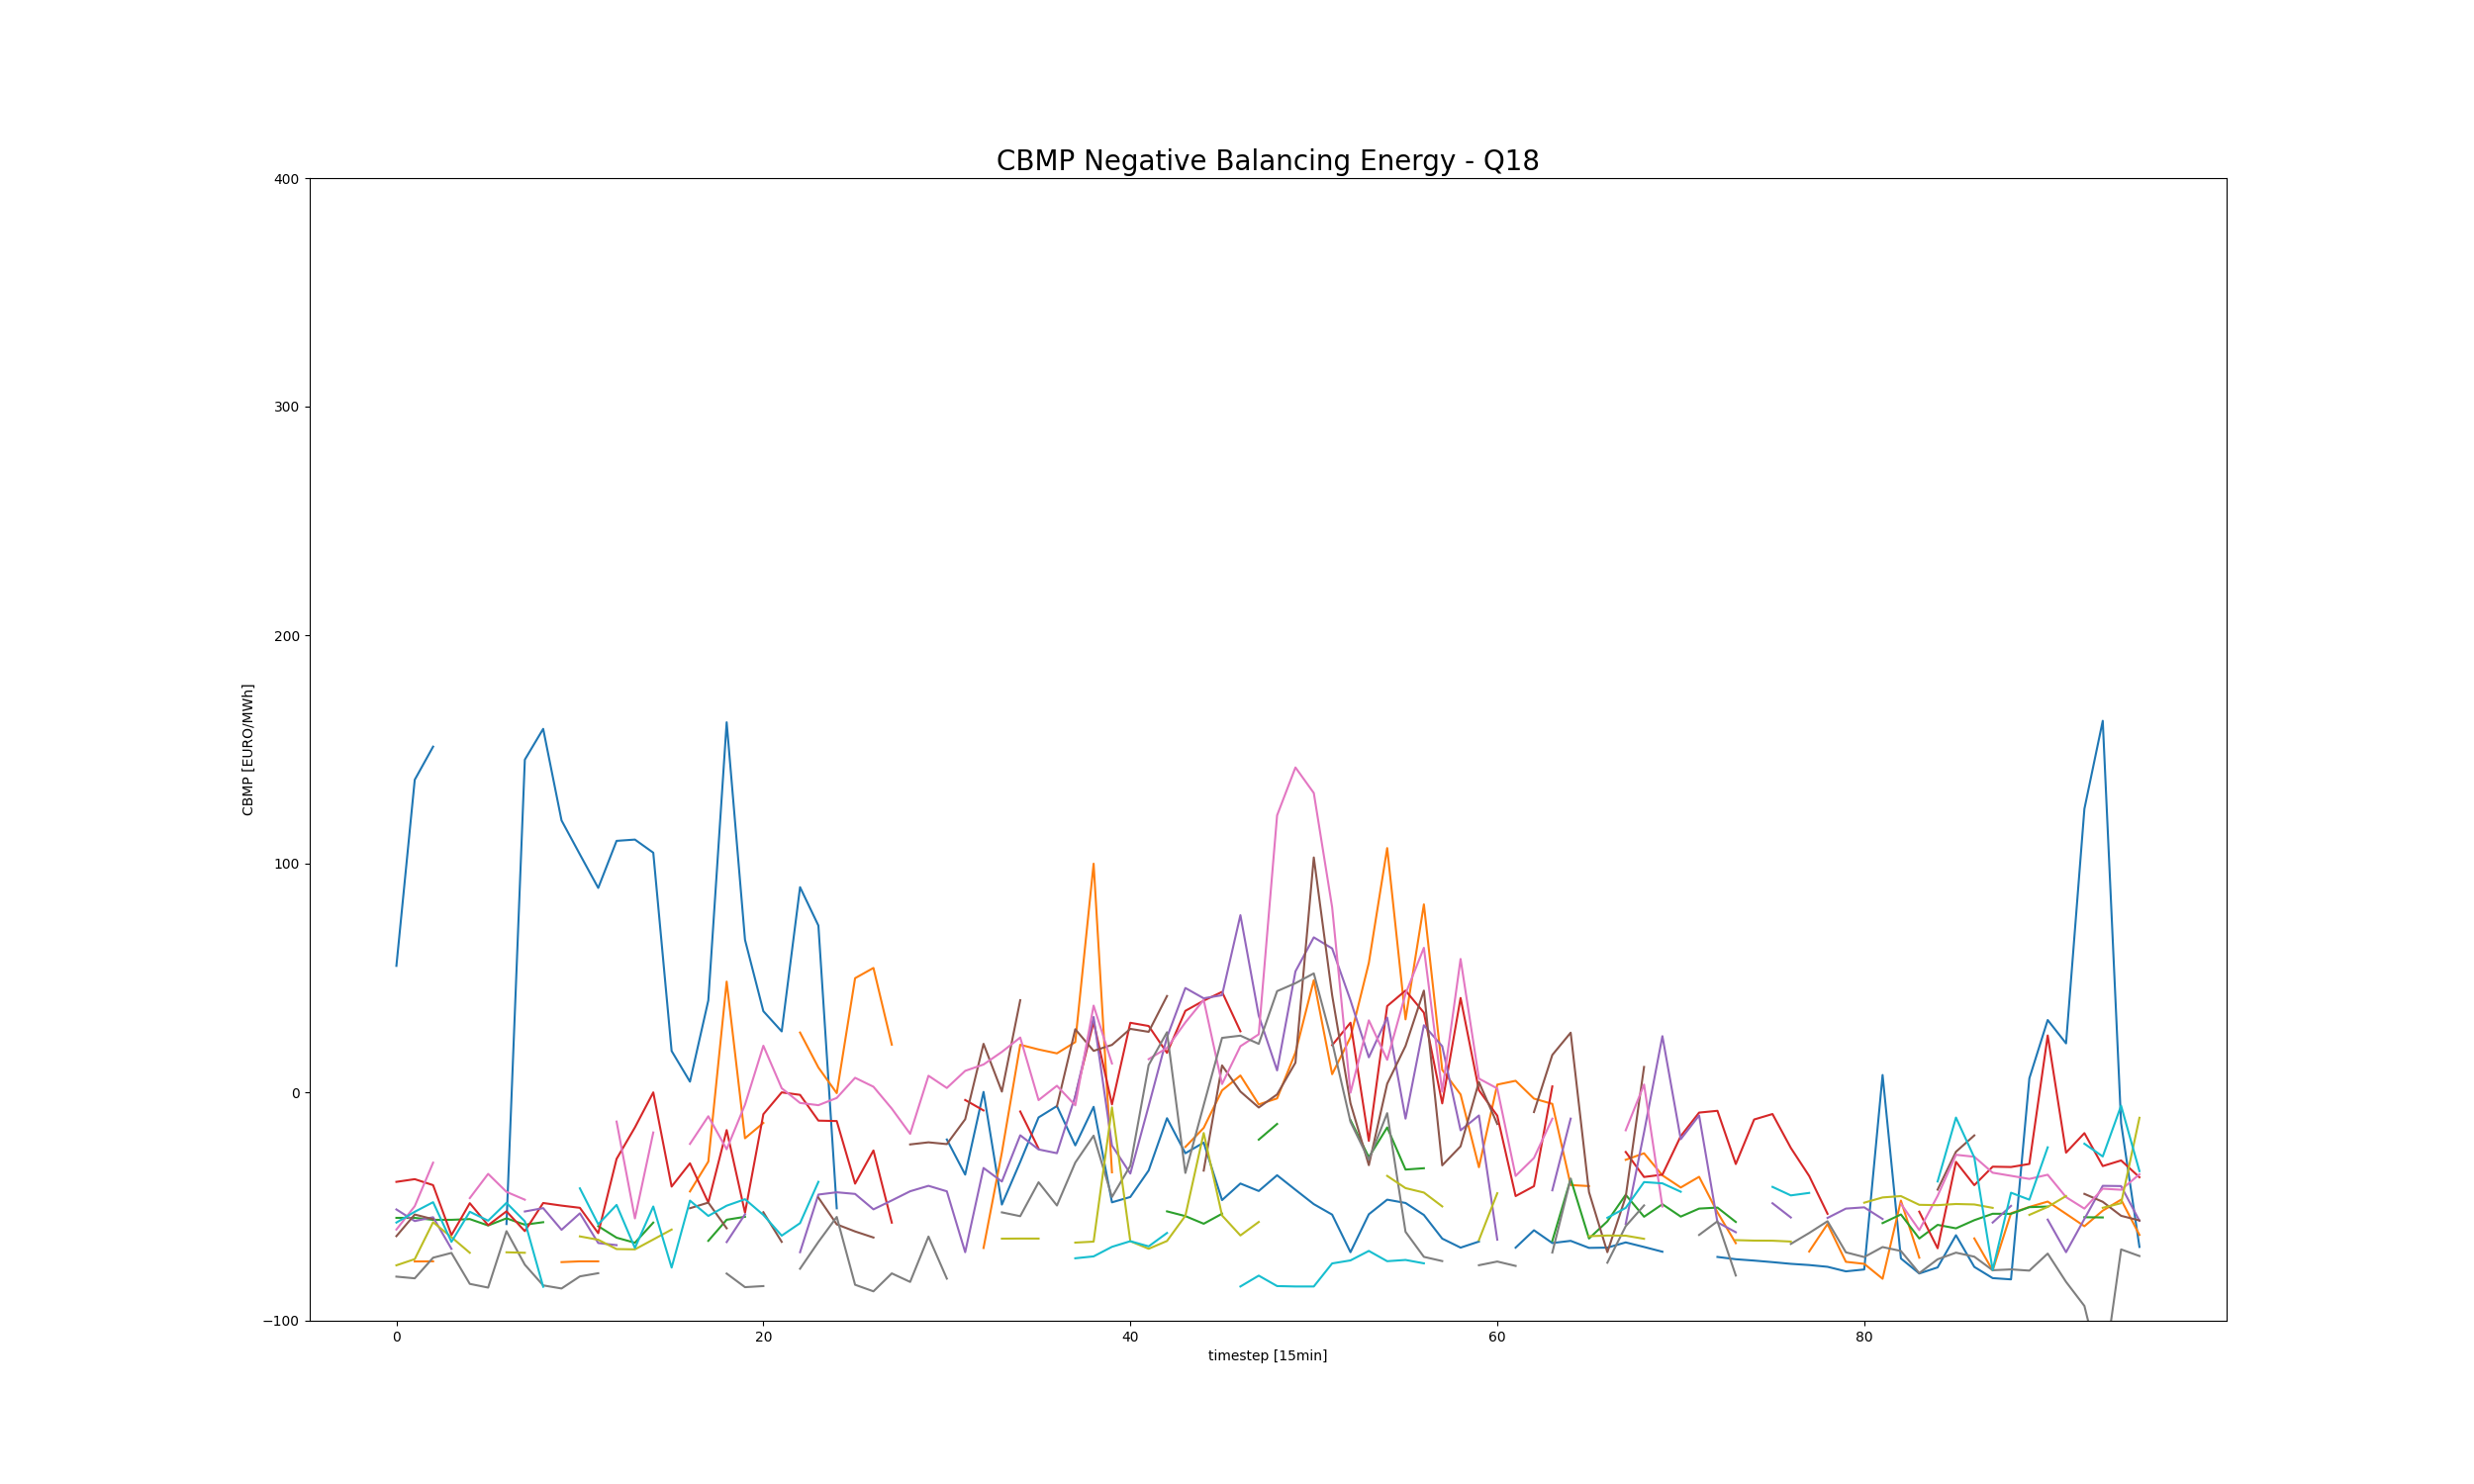
\includegraphics[width=1\linewidth]{pictures/results/CBMP_negBal_Q18.png}
	\caption{CBMP Negative Energy Q18}
	\label{fig:CBMP_negBal_Q18}
\end{figure}


\begin{figure}[H]
	\centering
	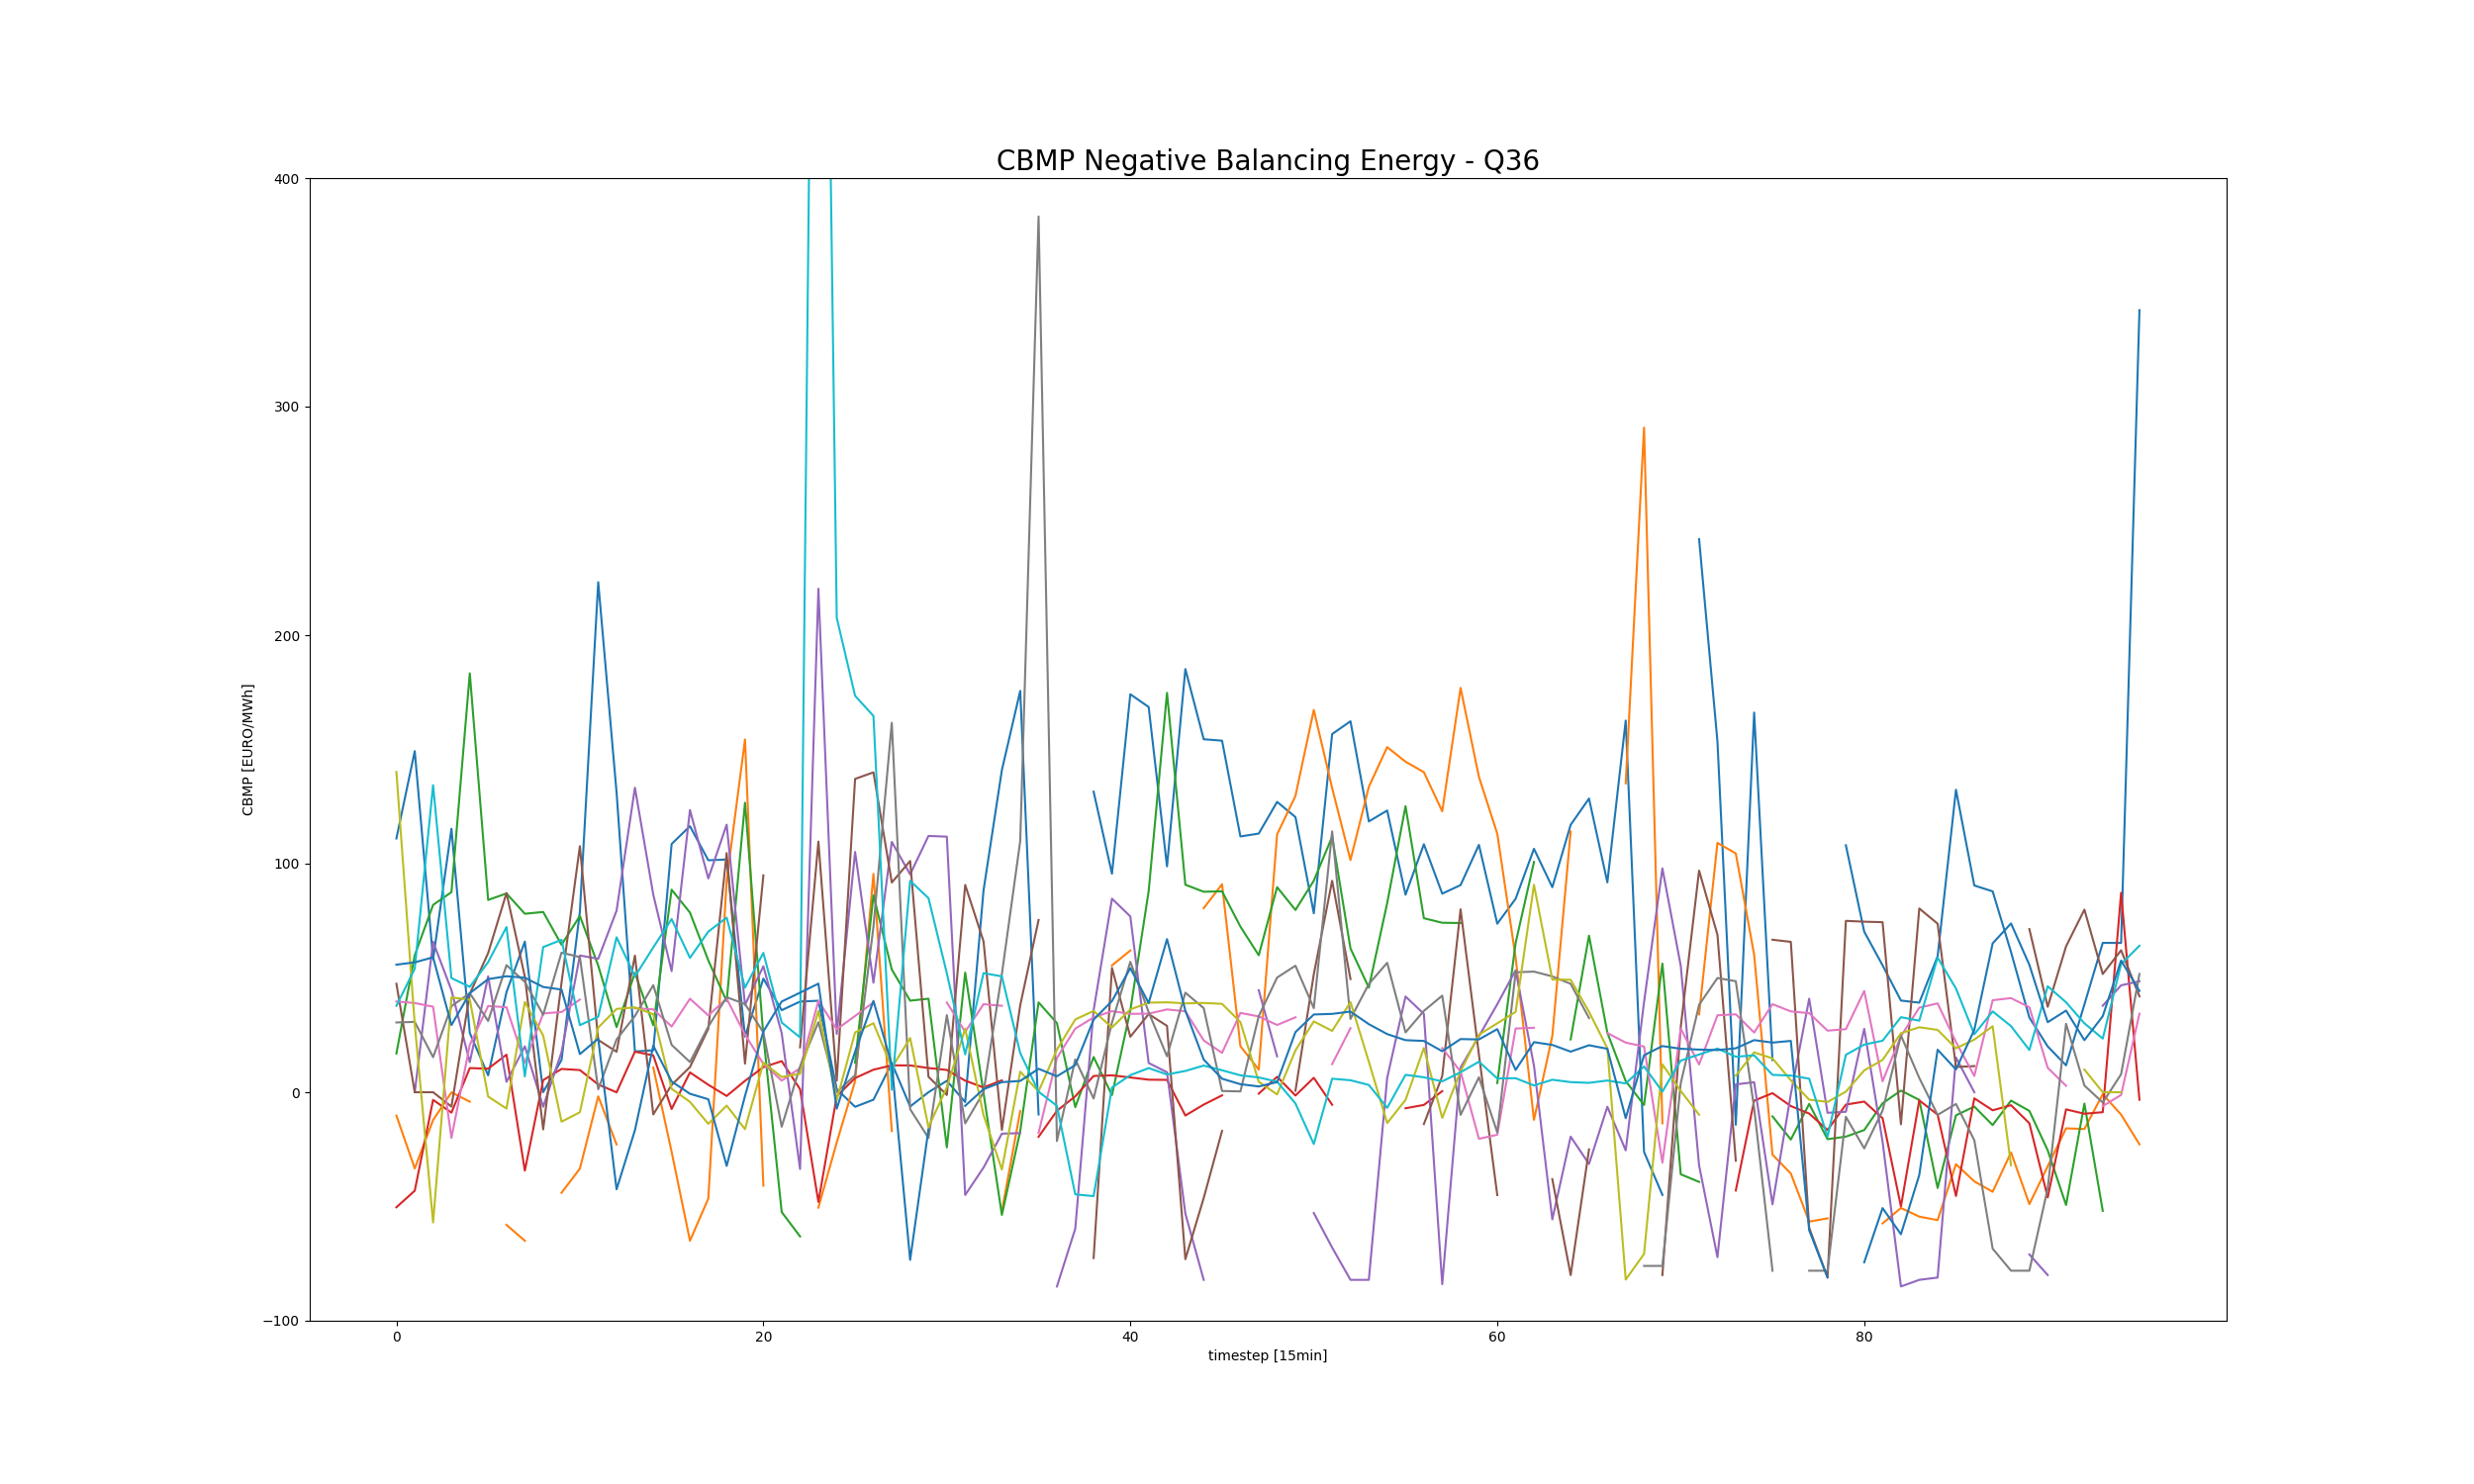
\includegraphics[width=1\linewidth]{pictures/results/CBMP_negBal_Q36.png}
	\caption{CBMP Negative Energy Q36}
	\label{fig:CBMP_negBal_Q36}
\end{figure}

\begin{figure}
	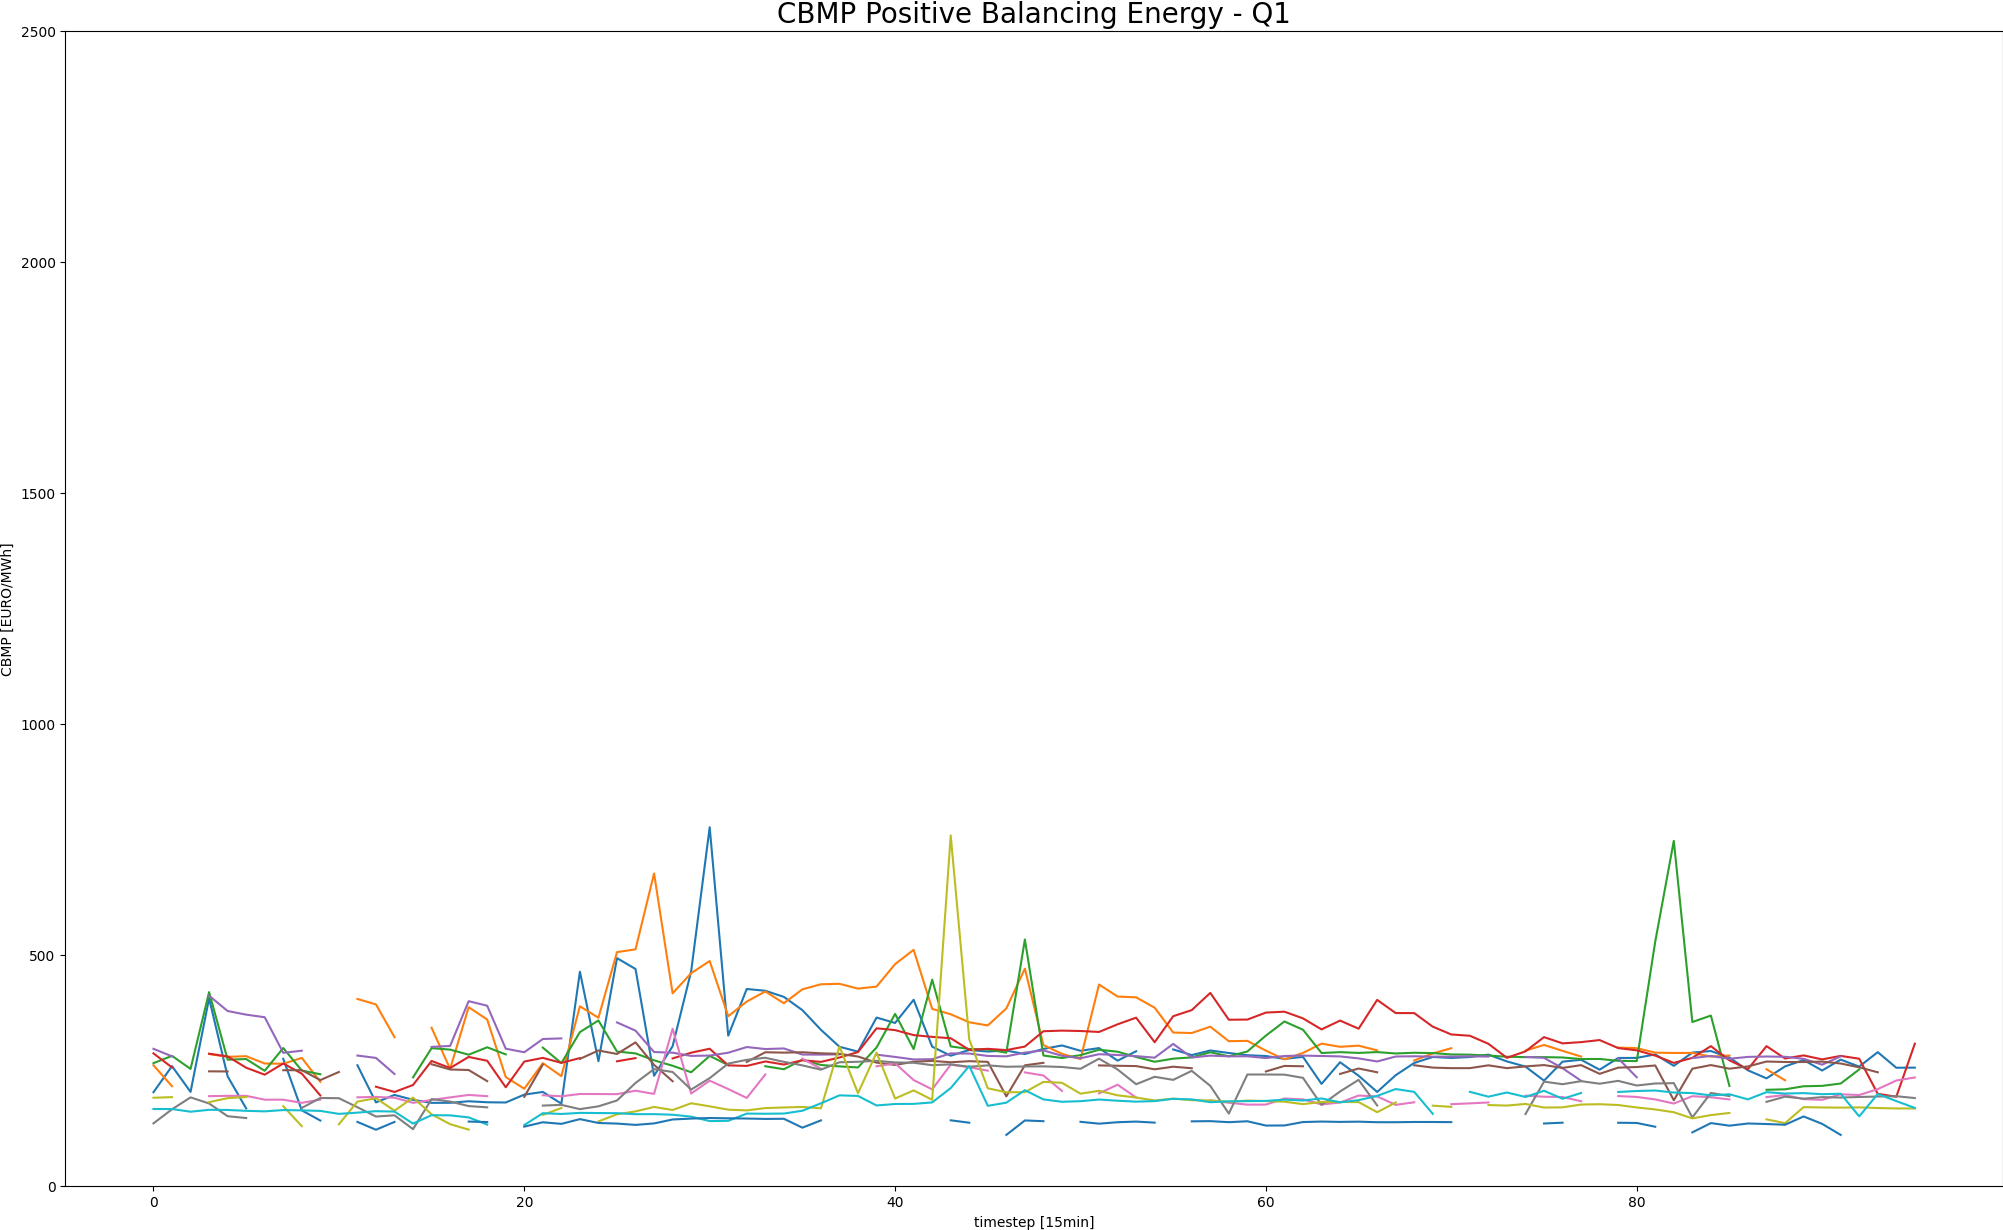
\includegraphics[width=1\linewidth]{pictures/results/CBMP_PosBal_Q1.png}
	\caption{CBMP Positive Energy Q1}
	\label{fig:CBMP_PosBal_Q1}
\end{figure}

\begin{figure}
	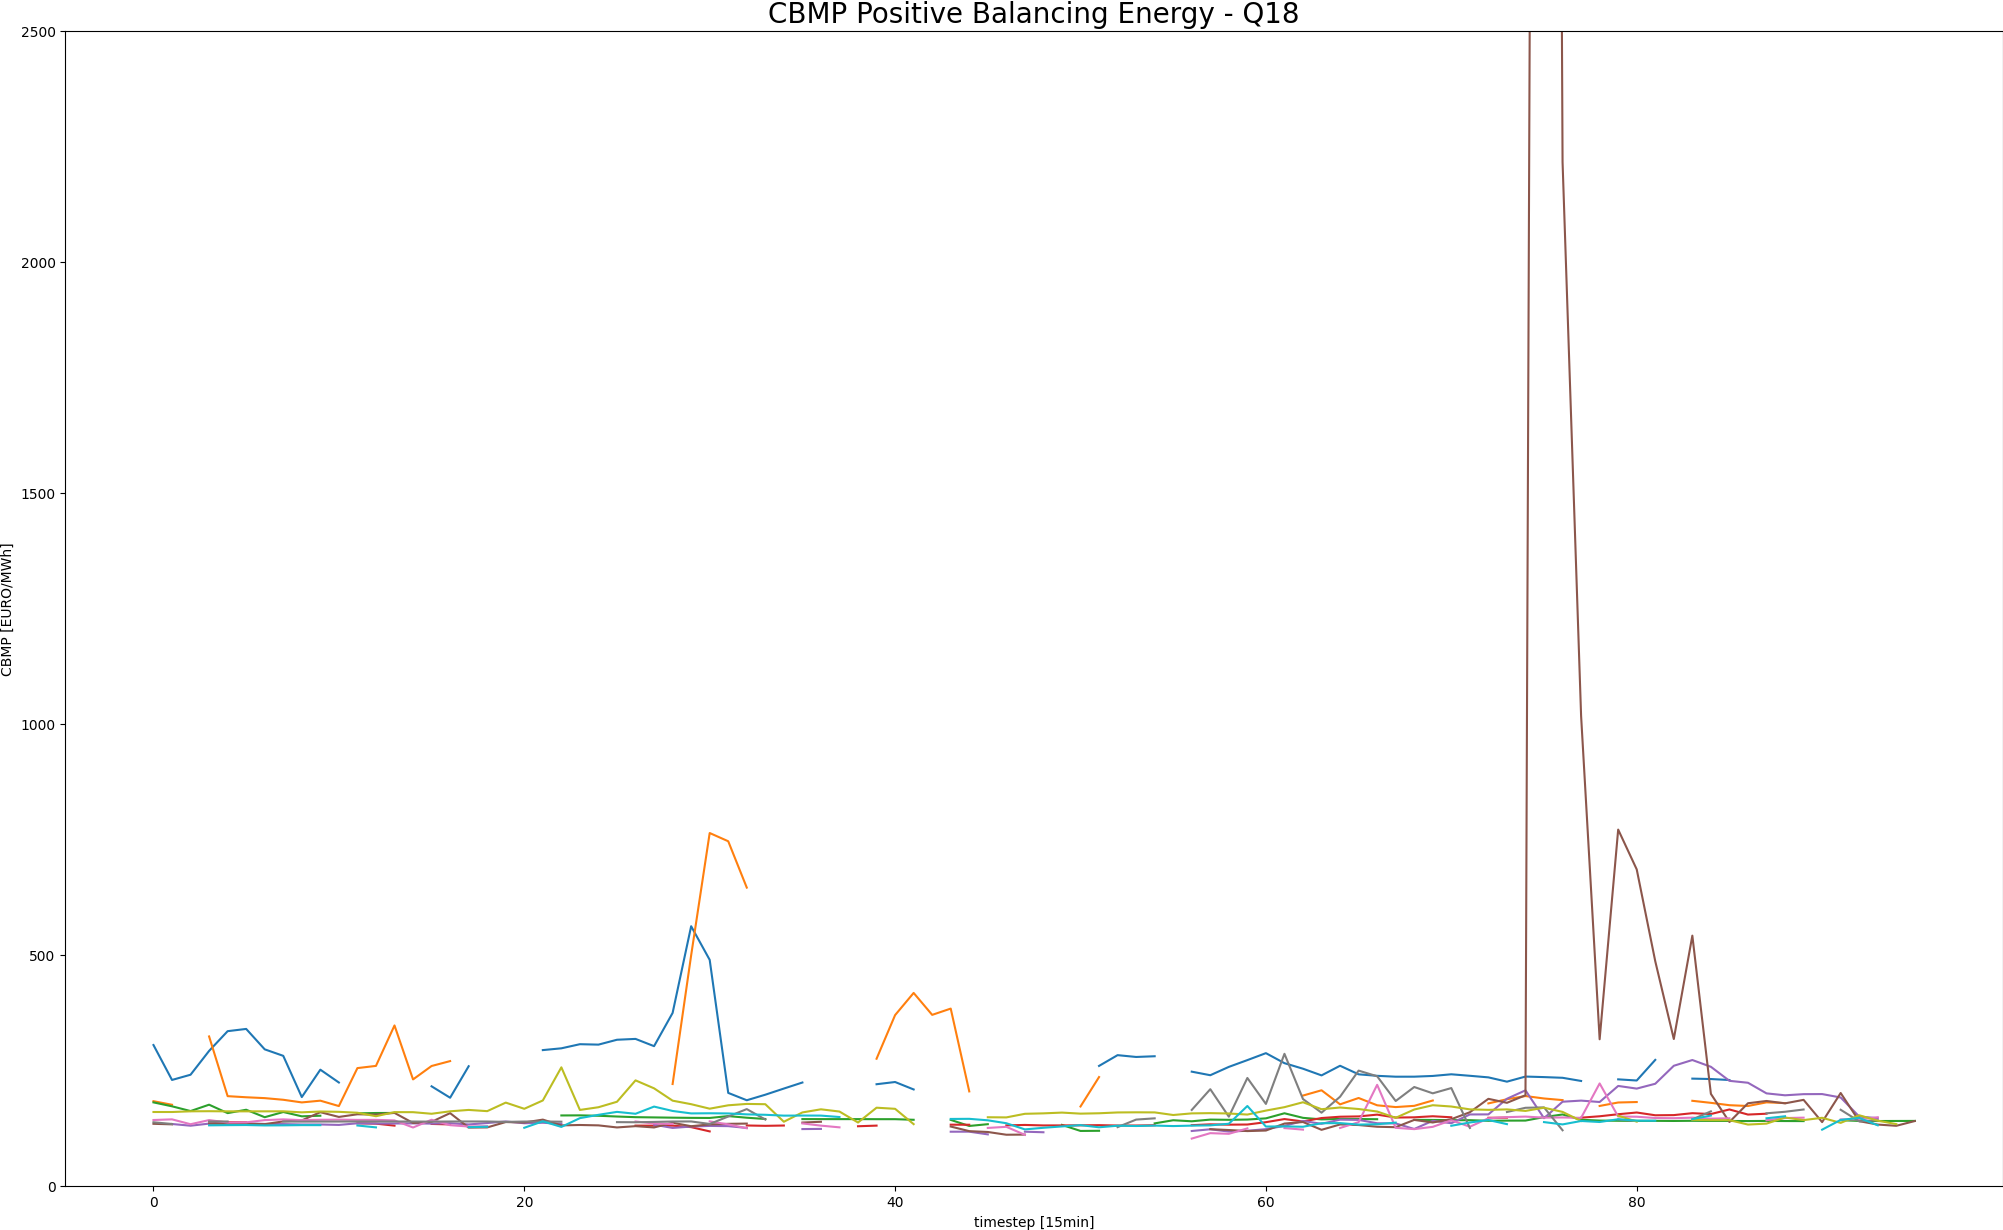
\includegraphics[width=1\linewidth]{pictures/results/CBMP_PosBal_Q18.png}
	\caption{CBMP Positive Energy Q18}
	\label{fig:CBMP_PosBal_Q18}
\end{figure}
\begin{figure}
	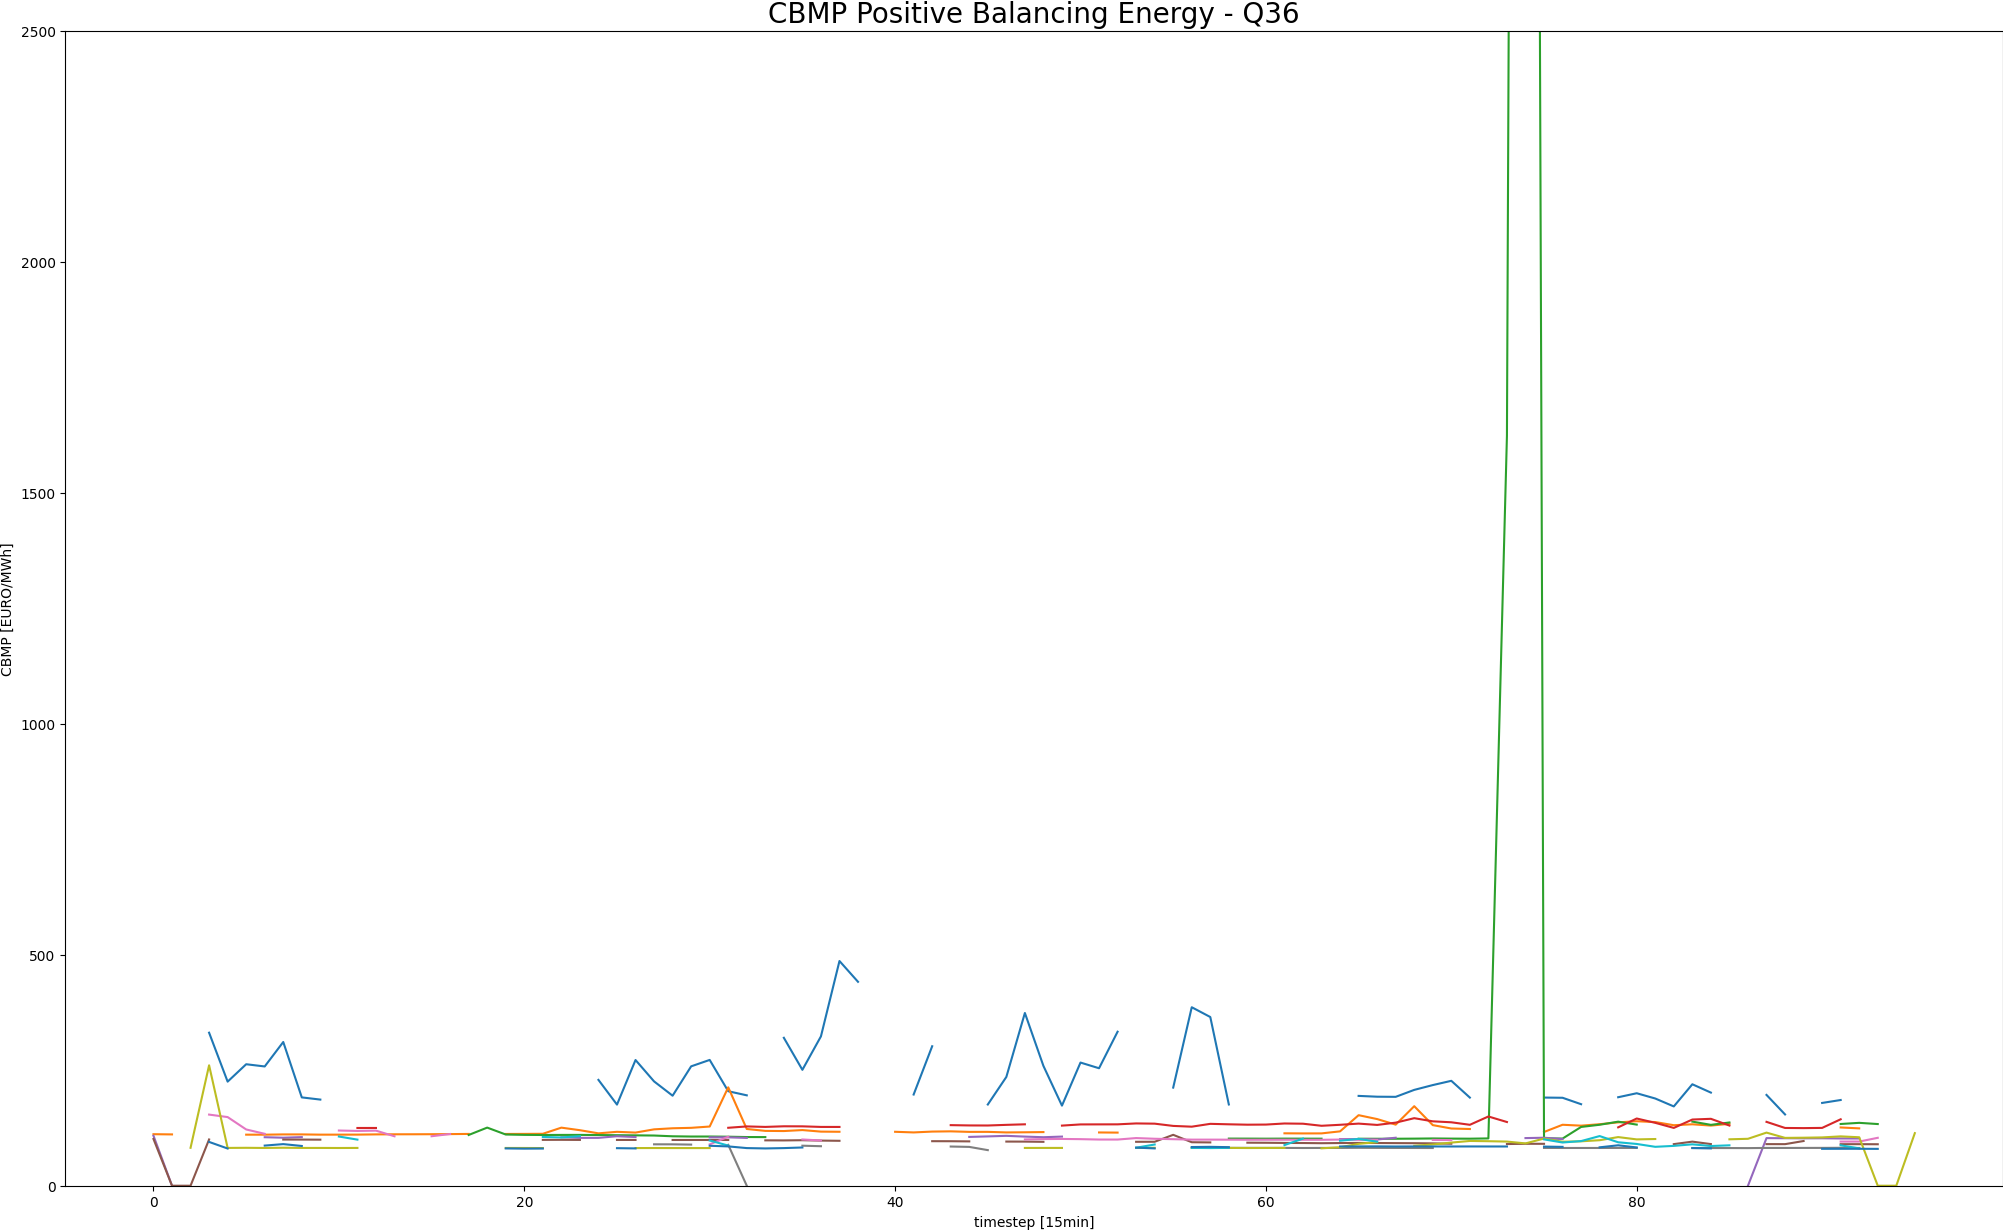
\includegraphics[width=1\linewidth]{pictures/results/CBMP_PosBal_Q36.png}
	\caption{CBMP Positive Energy Q36}
	\label{fig:CBMP_PosBal_Q36}
\end{figure}

Für den selben Zeitabschnitt lässt sich der DA Markt wie folgt zusammenfassen:
\begin{figure}[H]
	\centering
	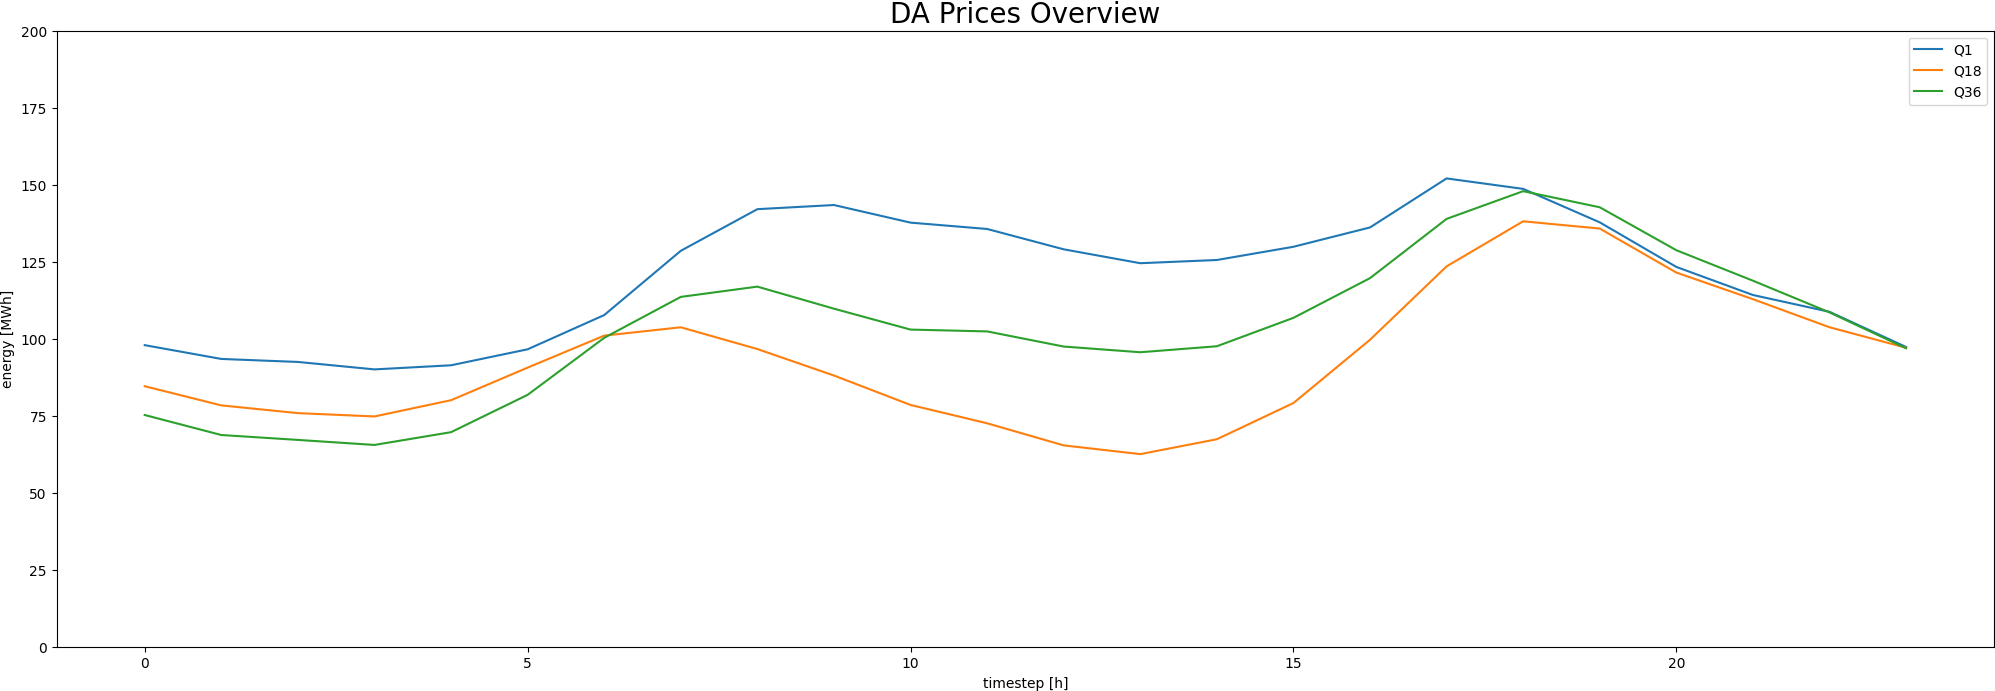
\includegraphics[width=1\linewidth]{pictures/results/DAPrices.png}
	\caption{DA Prices}
	\label{fig:DAPrices}
\end{figure}
\begin{figure}
	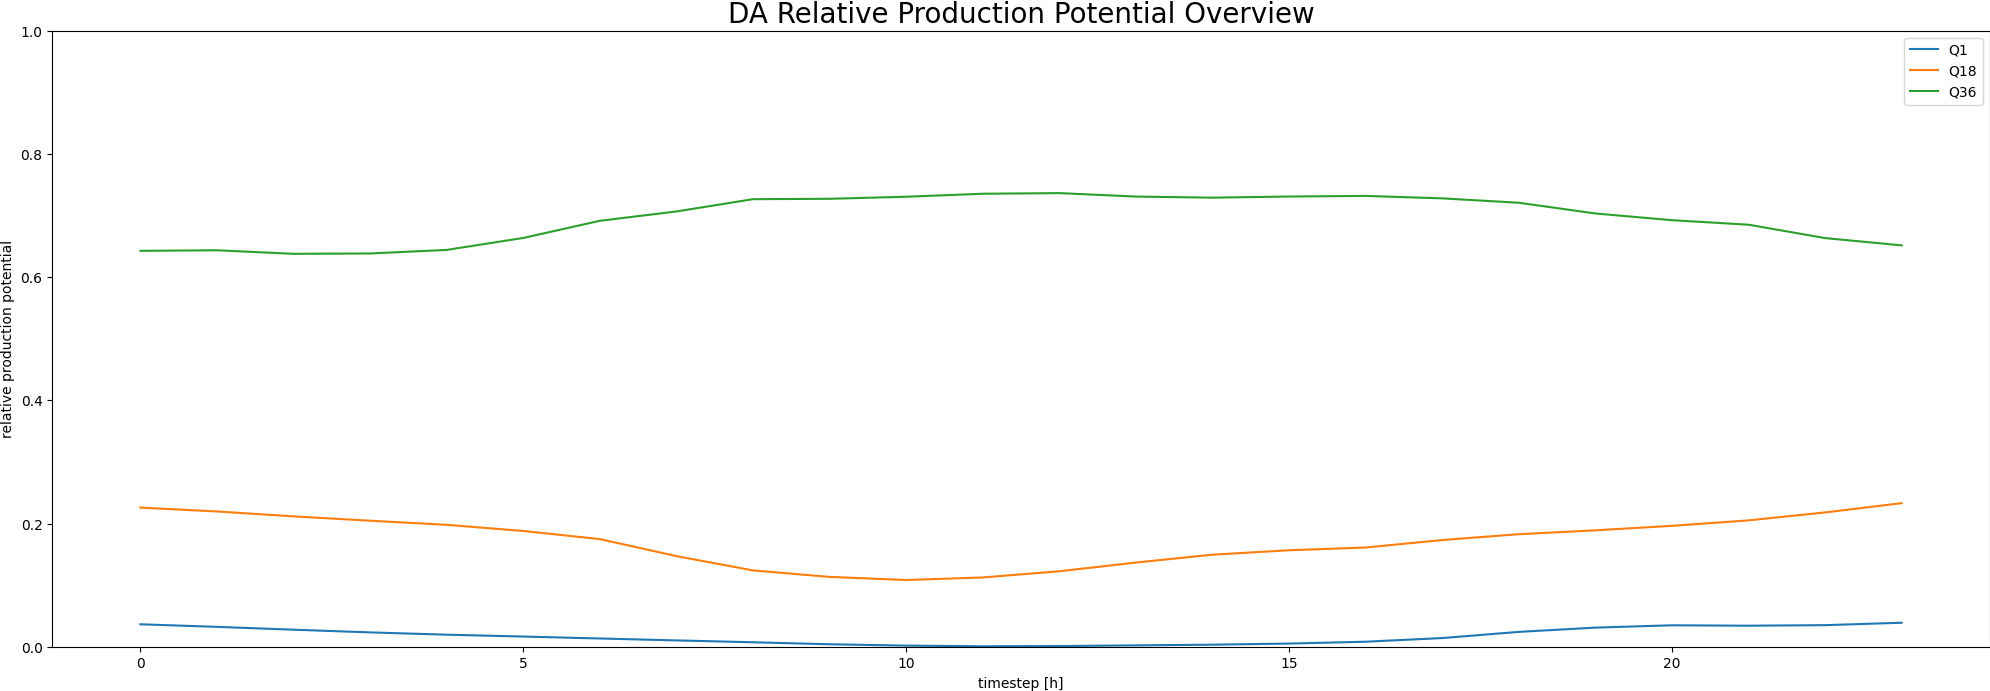
\includegraphics[width=1\linewidth]{pictures/results/DAProd.png}
	\caption{DA Production}
	\label{fig:DAProd}
\end{figure}

Außerdem stellt sich der entsprechende RL Markt wie folgt dar:

\begin{figure}[H]
	\centering
	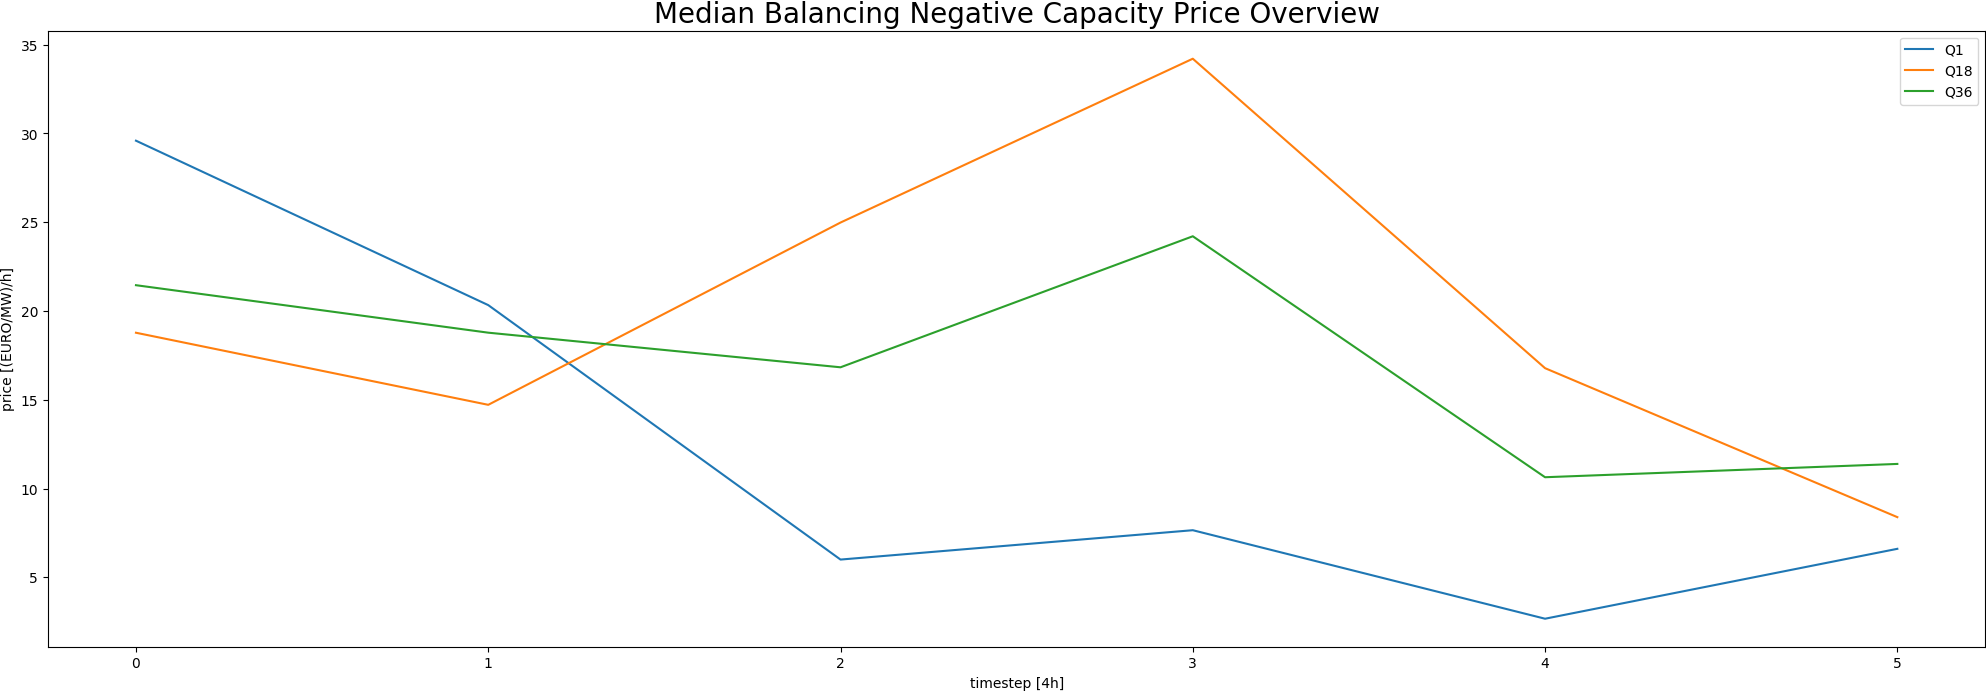
\includegraphics[width=1\linewidth]{pictures/results/RL_negPrice_Overview.png}
	\caption{RL Negative Prices}
	\label{fig:RL_negPrice_Overview}
\end{figure}
\begin{figure}
	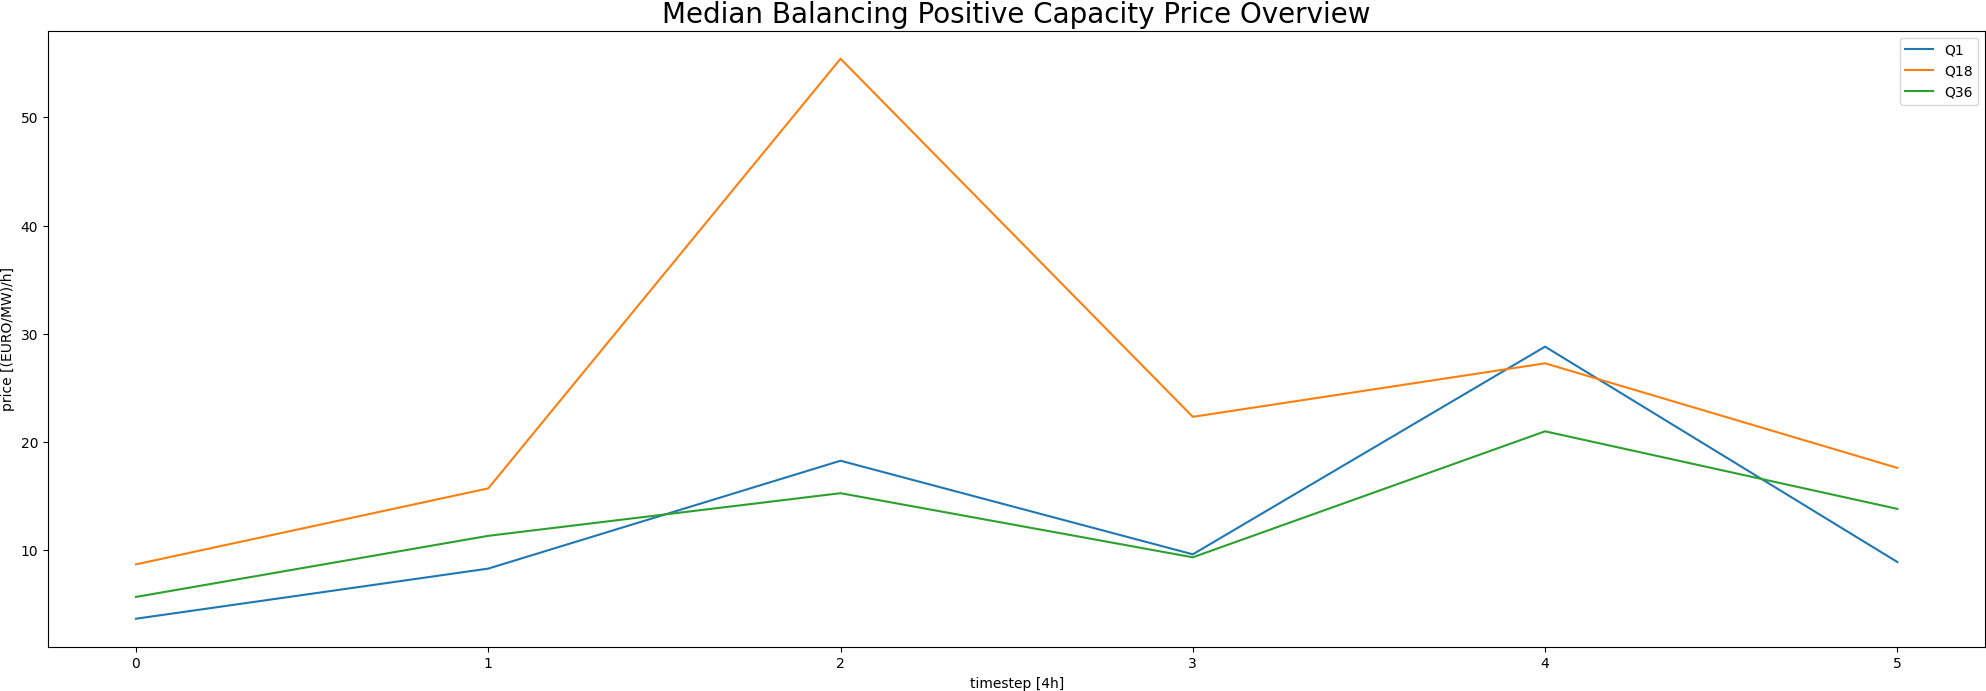
\includegraphics[width=1\linewidth]{pictures/results/RL_posPrice_Overview.png}
	\caption{RL Negative Prices}
	\label{fig:RL_posPrice_Overview}
\end{figure}

\section{Model Results}

\begin{figure}[H]
	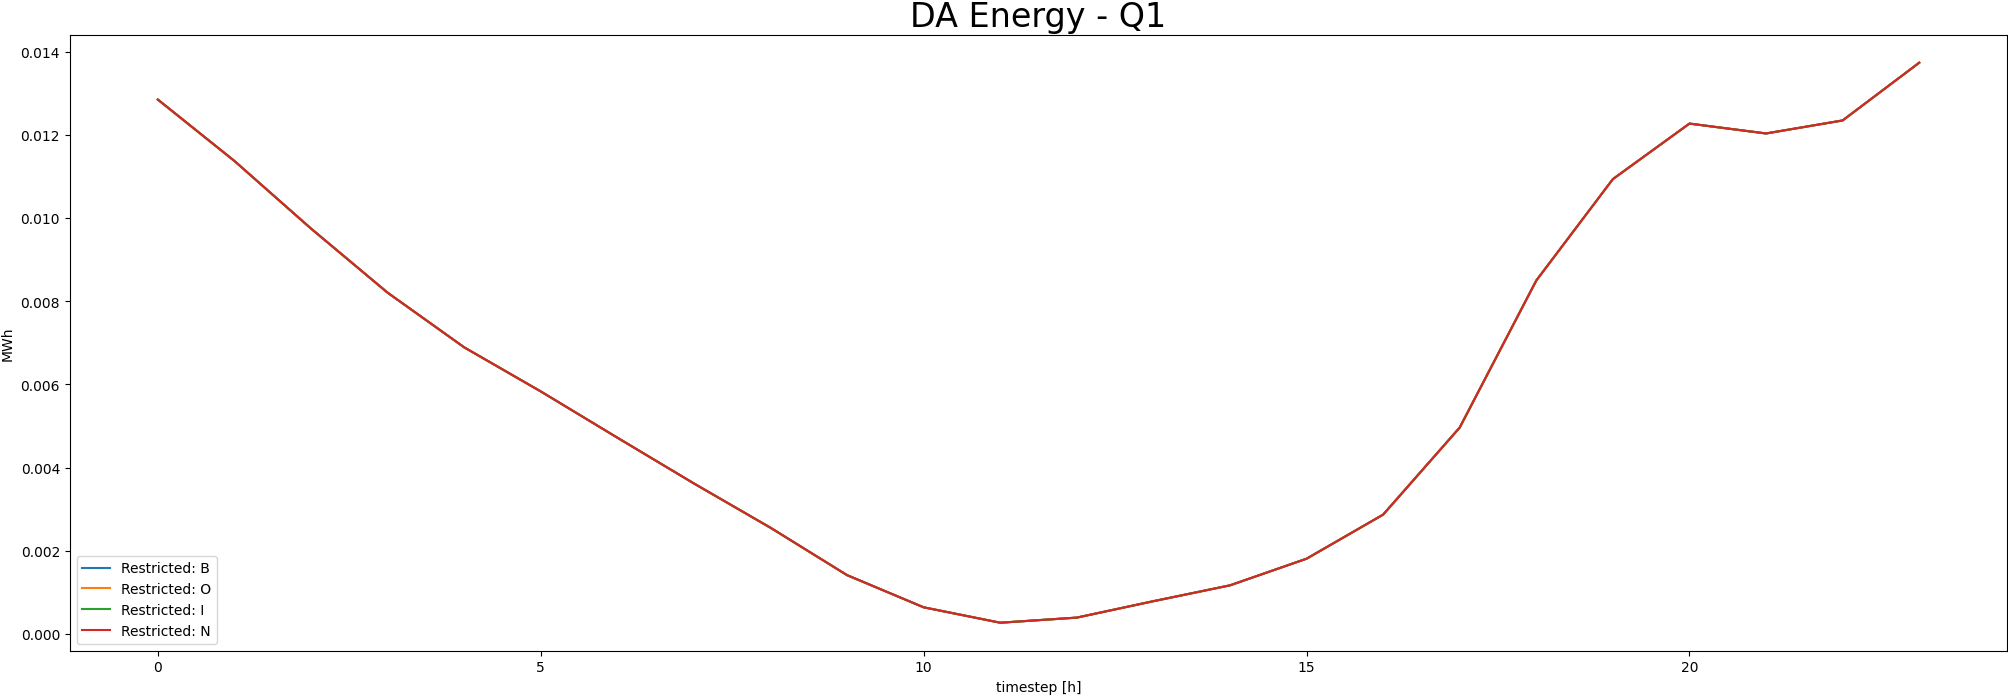
\includegraphics[width=1\linewidth]{pictures/results/DA Energy - Q1.png}
	\caption{DA Energy - Q1}
	\label{fig:DA Energy - Q1}
\end{figure}

\begin{figure}[H]
	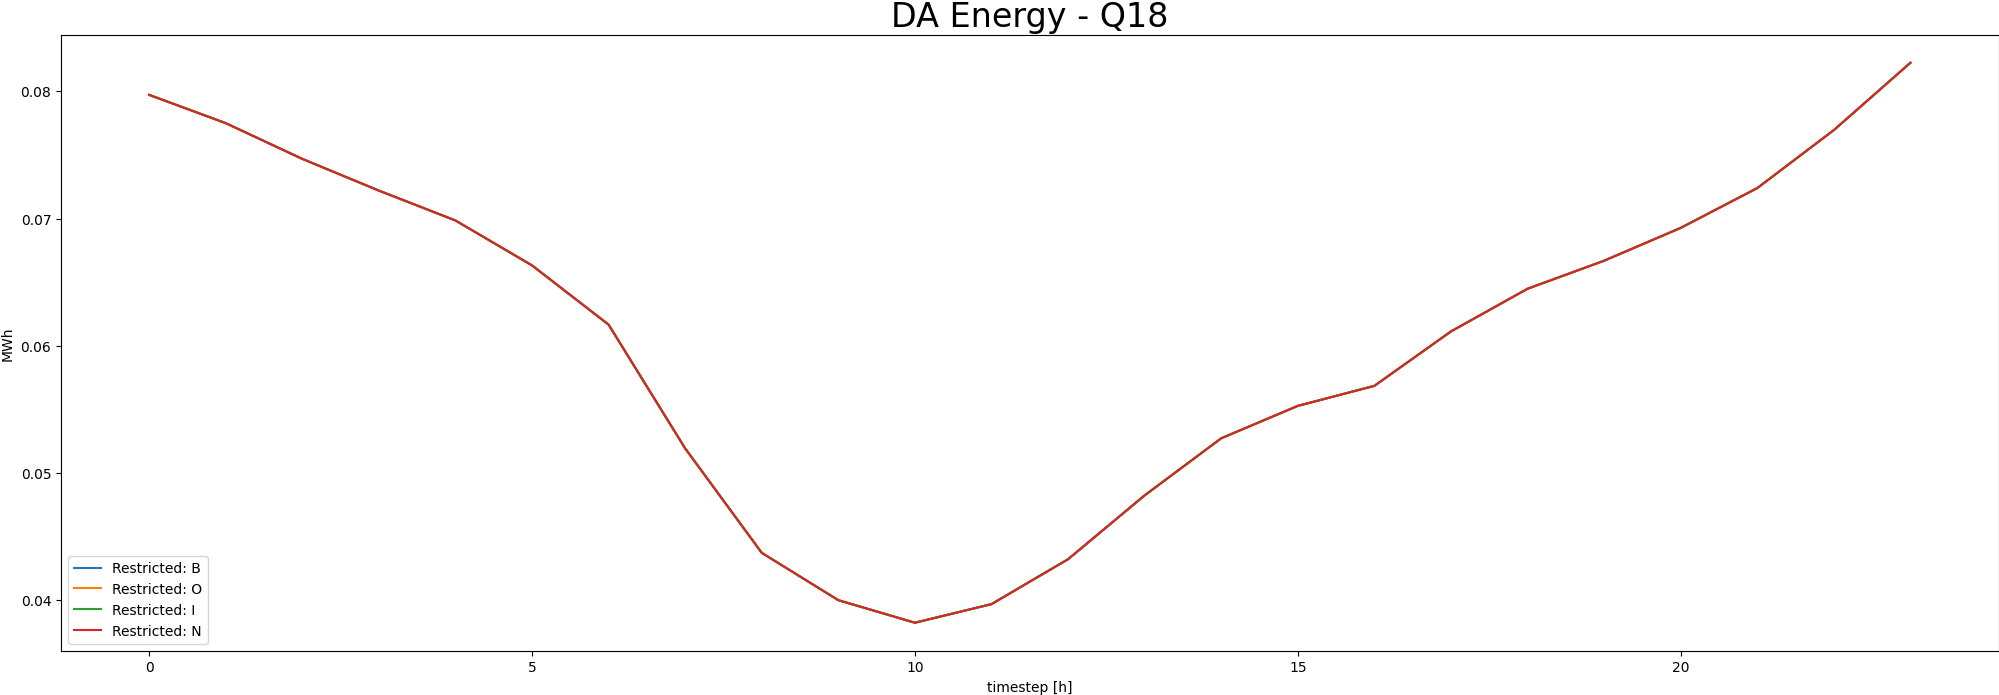
\includegraphics[width=1\linewidth]{pictures/results/DA Energy - Q18.png}
	\caption{DA Energy - Q18}
	\label{fig:DA Energy - Q18}
\end{figure}

\begin{figure}[H]
	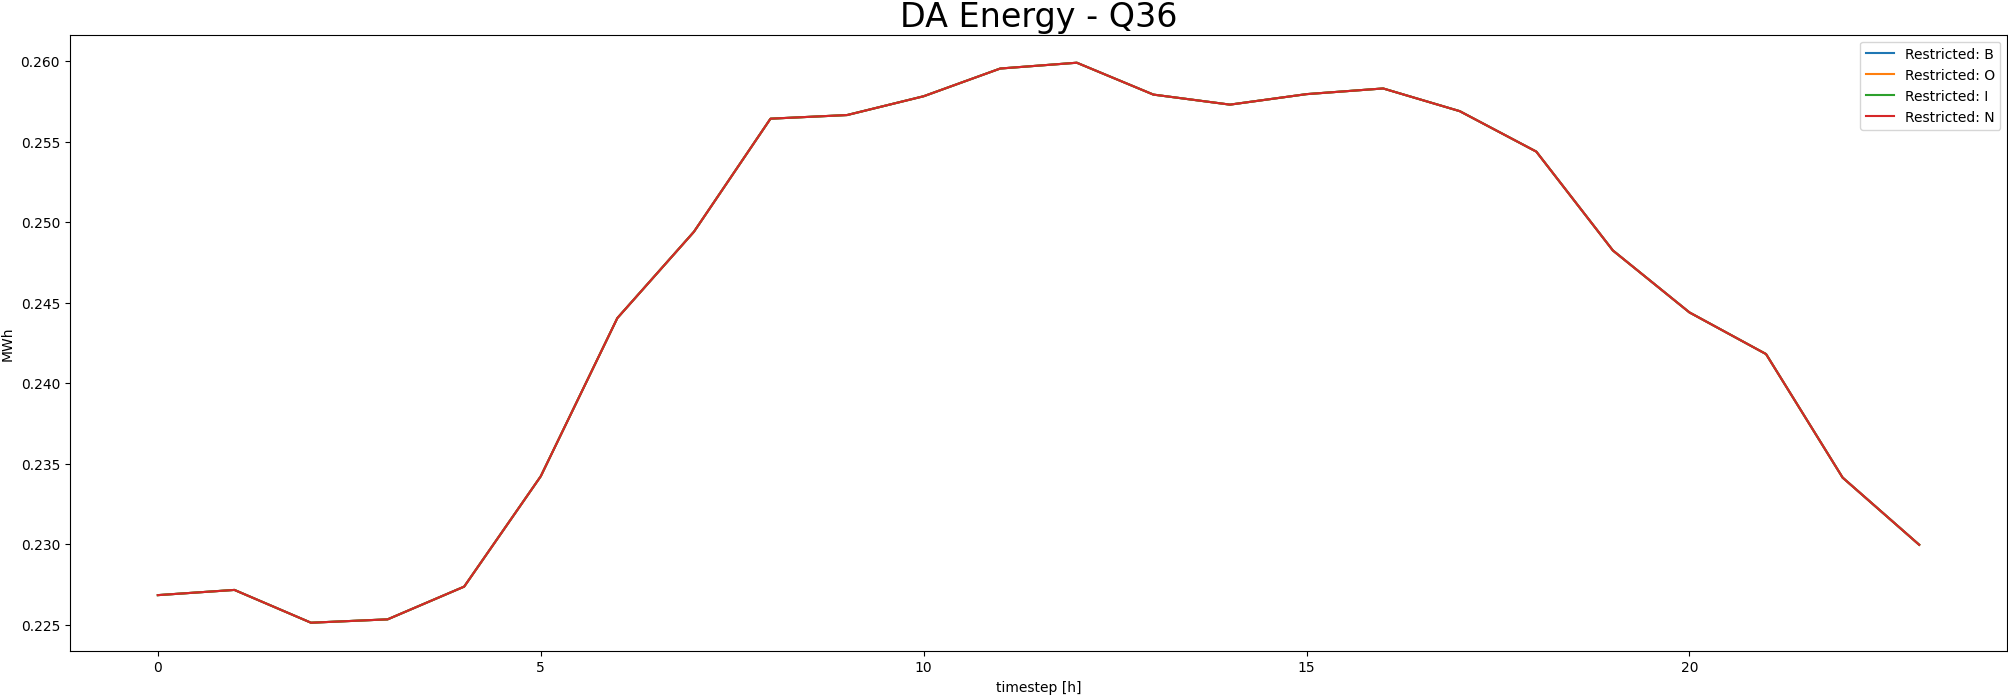
\includegraphics[width=1\linewidth]{pictures/results/DA Energy - Q36.png}
	\caption{DA Energy - Q36}
	\label{fig:DA Energy - Q36}
\end{figure}
\begin{figure}[H]
	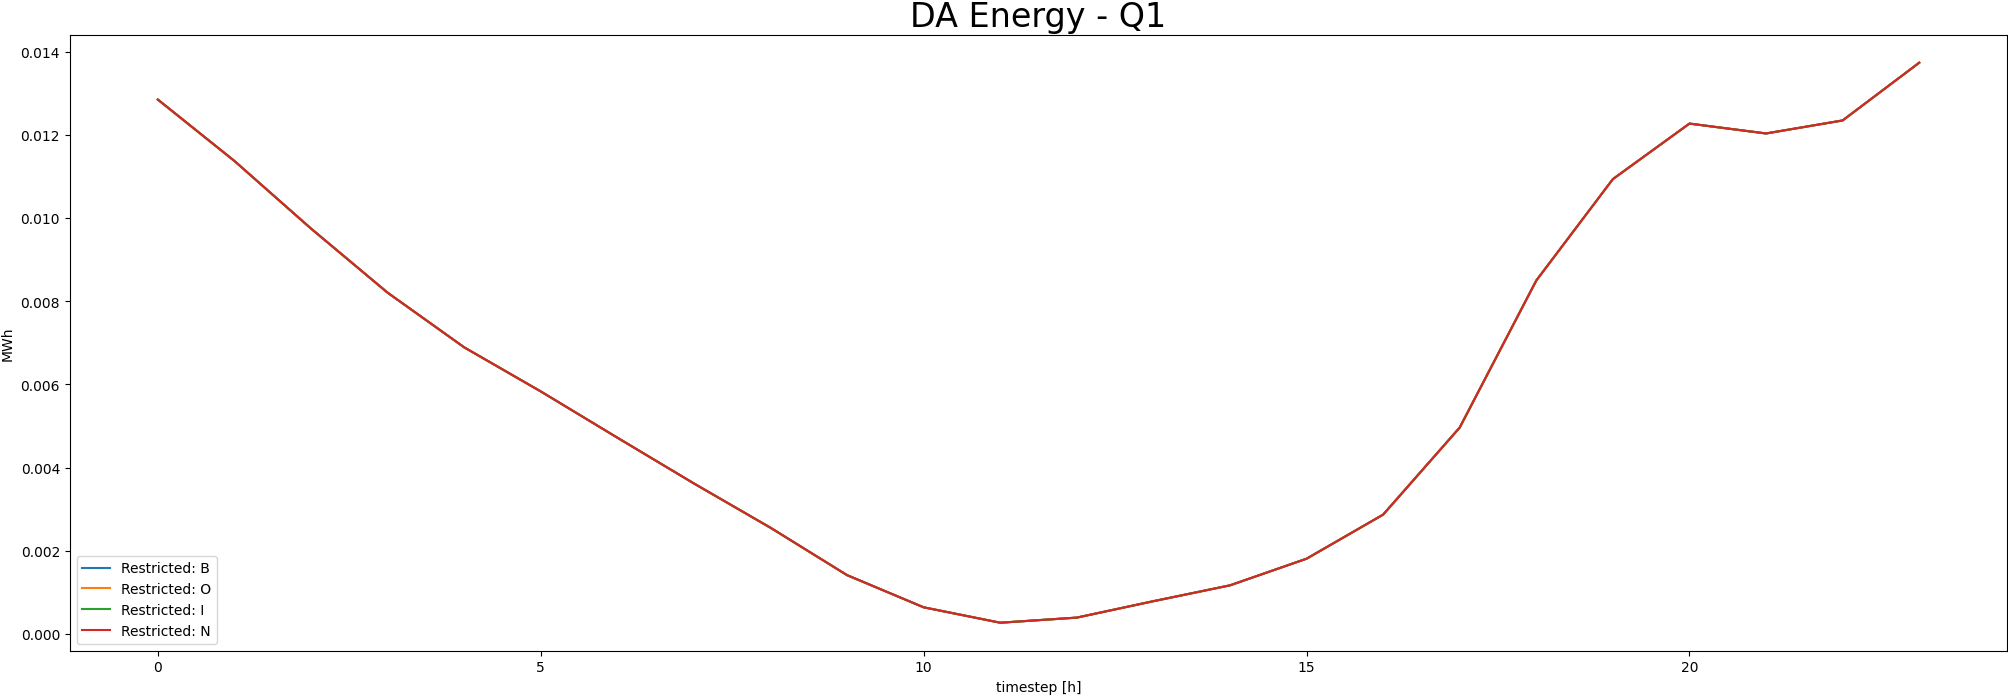
\includegraphics[width=1\linewidth]{pictures/results/DA Energy - Q1.png}
	\caption{Balance Capacity - Q1}
	\label{fig:Balance Capacity - Q1}
\end{figure}

\begin{figure}[H]
	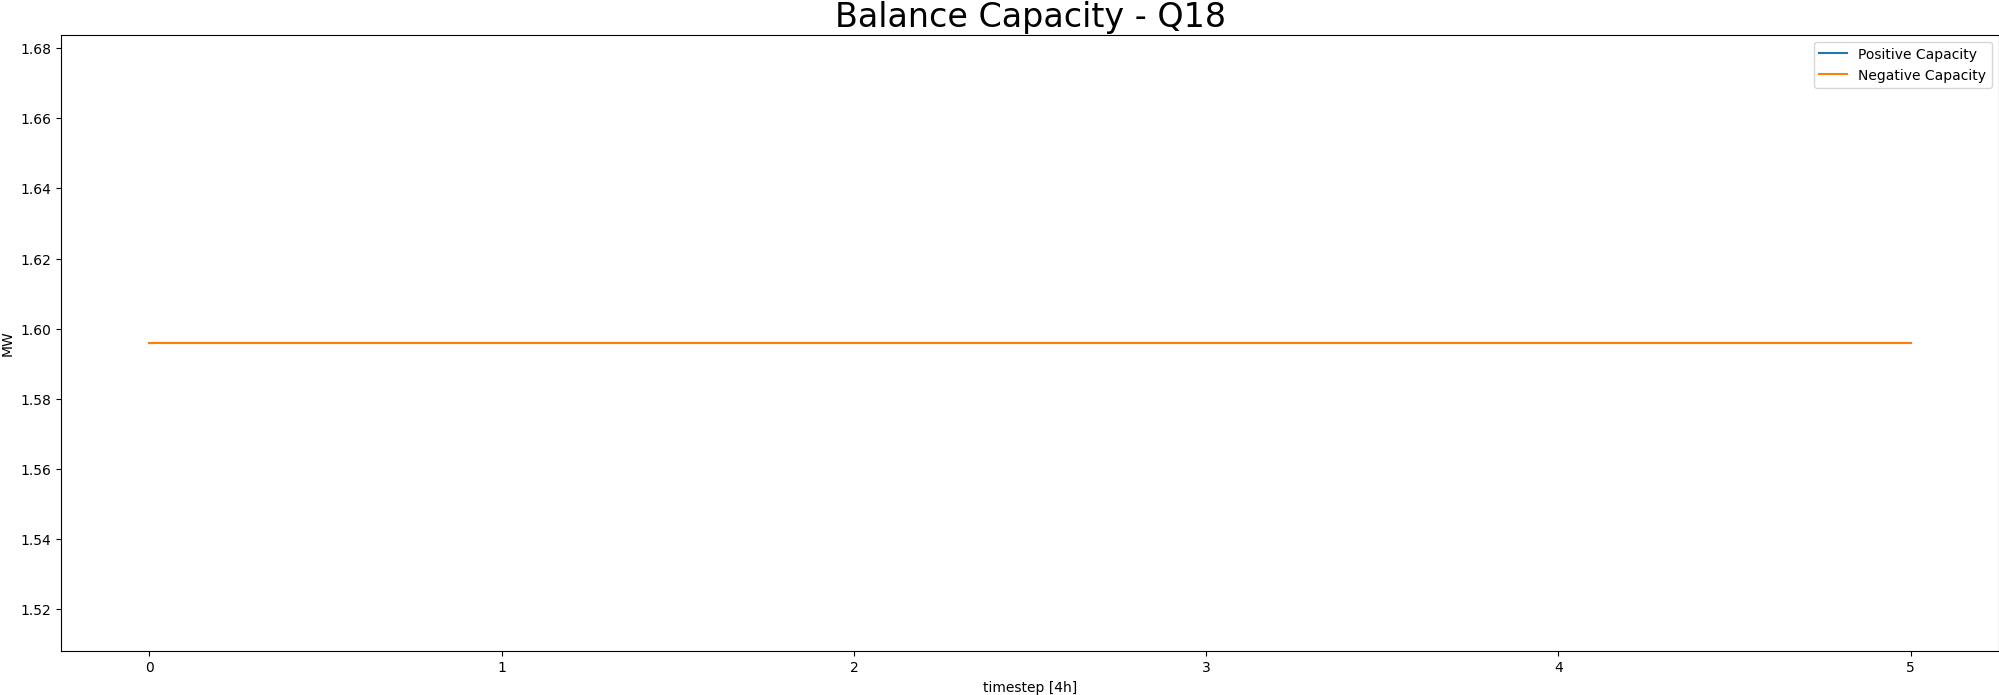
\includegraphics[width=1\linewidth]{pictures/results/Balance Capacity - Q18.png}
	\caption{Balance Capacity - Q18}
	\label{fig:Balance Capacity - Q18}
\end{figure}

\begin{figure}[H]
	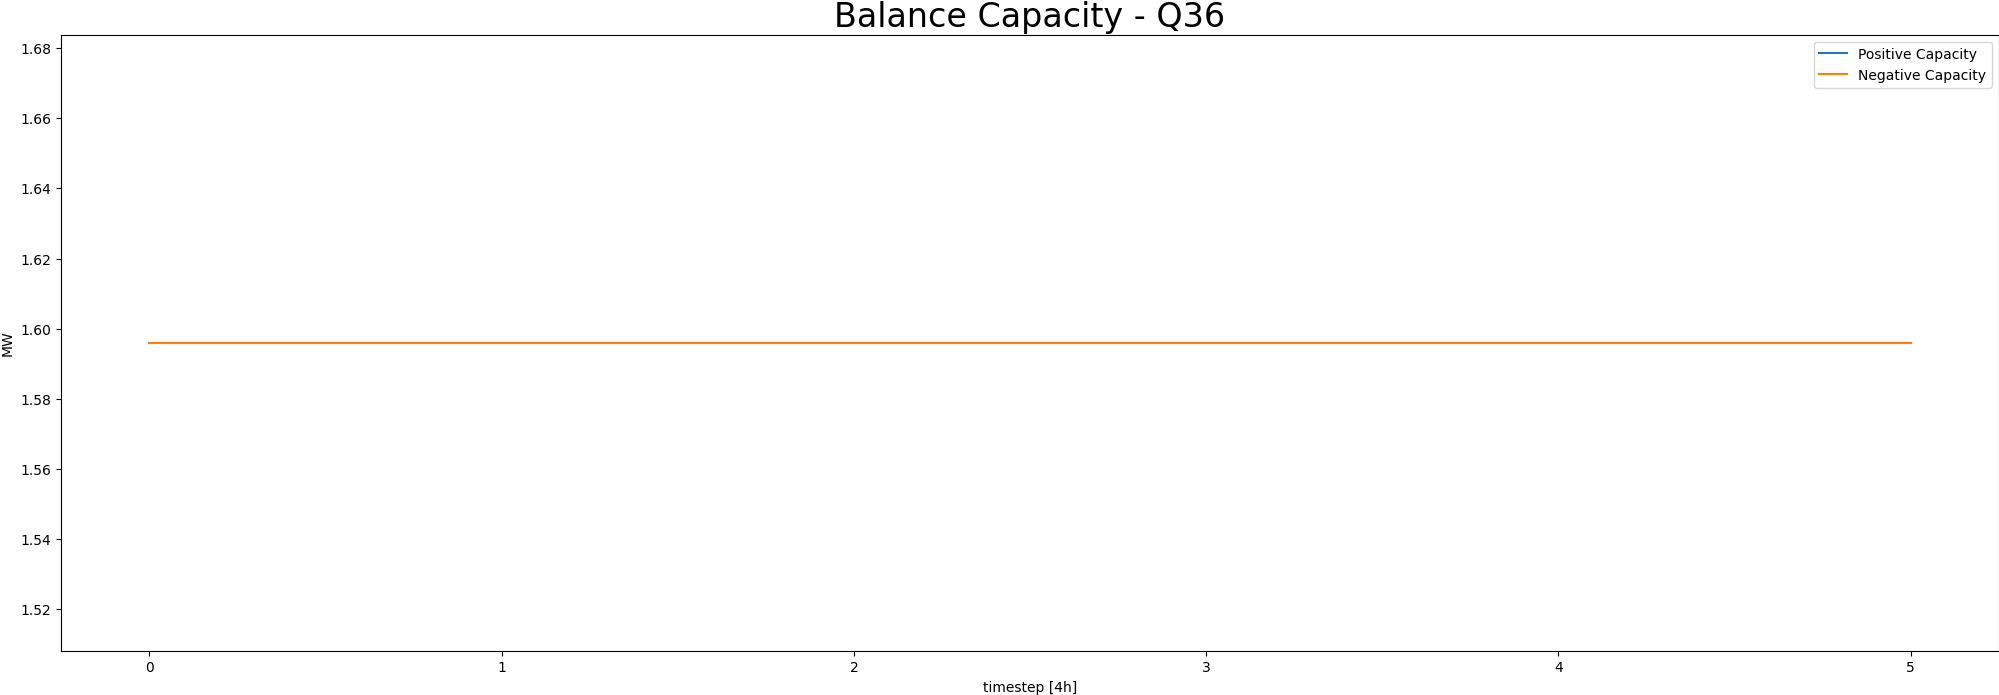
\includegraphics[width=1\linewidth]{pictures/results/Balance Capacity - Q36.png}
	\caption{Balance Capacity - Q36}
	\label{fig:Balance Capacity - Q36}
\end{figure}







\section{Digital Appendix}



%% *** local page settings ***
\addtocontents{toc}{\protect\setcounter{tocdepth}{+1}} %reset the decreased depth of the appendix entry in the ToC
\label{subsec:Bibliography}
\printbibliography[title={Bibliography}]
%% change chapter title to german if necessary



ChatGPT was utilized in this work for the following purposes:
\begin{itemize}
	\item As a search tool for specific functions.
	\item As an aid in refining formulations.
\end{itemize}
All suggestions were carefully reviewed and assessed individually.



\begin{center}
	\textbf{Statement of authorship}
\end{center}

I hereby certify that I have authored this document entitled "Model-based analysis of various
marketing options on the german secondary balancing market for a large-scale storage facility" independently
and without undue assistance from third parties. No other than the resources and references
indicated in this document have been used. I have marked both literal and accordingly adopted
quotations as such. There were no additional persons involved in the intellectual preparation
of the present document. I am aware that violations of this declaration may lead to subsequent
withdrawal of the academic degree.\\

\begin{figure}[!h]
	
\includegraphics[width=0.5\linewidth]{figures/unterschrift.png}
\end{figure}
Dresden, 20th April 2025\\
Sebastian Trümper\\




\end{document}
